% ------------------------------------------------------------------------
% ------------------------------------------------------------------------
% Artigo Projeto Integrador -PI4
%
% ------------------------------------------------------------------------
% ------------------------------------------------------------------------

\documentclass[
	% -- opções da classe memoir --
	article,			% indica que é um artigo acadêmico
	11pt,				% tamanho da fonte
	oneside,			% para impressão apenas no recto. Oposto a twoside
	a4paper,			% tamanho do papel.
	% -- opções da classe abntex2 --
	%chapter=TITLE,		% títulos de capítulos convertidos em letras maiúsculas
	section=TITLE,		% títulos de seções convertidos em letras maiúsculas
	%subsection=Title,	% títulos de subseções convertidos em letras maiúsculas
	%subsubsection=TITLE % títulos de subsubseções convertidos em letras maiúsculas
	% -- opções do pacote babel --
	english,			% idioma adicional para hifenização
	brazil,				% o último idioma é o principal do documento
	sumario=tradicional
	]{abntex2}


% ---
% PACOTES
% ---

% ---
% Pacotes fundamentais 
% ---
\usepackage{lmodern}			% Usa a fonte Latin Modern
\usepackage[T1]{fontenc}		% Selecao de codigos de fonte.
\usepackage[utf8]{inputenc}		% Codificacao do documento (conversão automática dos acentos)
\usepackage{indentfirst}		% Indenta o primeiro parágrafo de cada seção.
\usepackage{color}				% Controle das cores
\usepackage{graphicx}			% Inclusão de gráficos
\usepackage{microtype} 			% para melhorias de justificação

%\usepackage{nomencl} 			% Lista de simbolos
\graphicspath{ {./images/} }
\usepackage{caption}
\usepackage{subcaption}
\usepackage{booktabs}
\usepackage{array}
\usepackage{multicol}
\usepackage{rotating}
\usepackage{tikz}
\usepackage{float}
\usepackage{makecell}
\usepackage{multicol}
%\usepackage{lipsum}
\usepackage{soul}
\usepackage{multirow}
%\usepackage[margin=1mm]{geometry}
%\geometry{a4paper, portrait, margin=0.5cm}
\usepackage{pdflscape}
\usepackage{amsmath}
\usepackage{amssymb}
\usepackage{pgfplots}
%\usepackage{pdfpages}
\usepackage{float}
\usepackage{makecell}
\usepackage{multicol}
\usepackage{subcaption}
\usepackage{minted}
%\usepackage{pgfplotstable}


\usepackage{tikz}
\usetikzlibrary{shapes,arrows}

\tikzstyle{block} = [draw, fill=white, rectangle, 
    minimum height=2.5em, minimum width=4em]
\tikzstyle{sum} = [draw, fill=white, circle, node distance=1cm]
\tikzstyle{input} = [coordinate]
\tikzstyle{output} = [coordinate]
\tikzstyle{pinstyle} = [pin edge={to-,thin,black}]

% ---

% ---
% Pacotes de citações
% ---
\usepackage[brazilian,hyperpageref]{backref}	 % Paginas com as citações na bibl
\usepackage[alf]{abntex2cite}	% Citações padrão ABNT
% ---

\newcommand{\nomeproduto}{\textit{Parvus Scala: \\ \large{Sistema de controle de nível}}}%
\newcommand{\diam}{$\varnothing$}%
\newcommand{\xPID}{130}%
\newcommand{\yPID}{1.2}%
\newcommand{\factorio}{\textit{Factory.io}}%
\newcommand{\EE}{Elipse E3}%
\newcommand{\Py}{\textit{Python}}%
\newcommand{\Mb}{\textit{Modbus}}%

\captionsetup[figure]{labelfont=small,textfont=small} %configura caption das imagens
% ---
% Configurações do pacote backref
% Usado sem a opção hyperpageref de backref
\renewcommand{\backrefpagesname}{Citado na(s) página(s):~}
% Texto padrão antes do número das páginas
\renewcommand{\backref}{}
% Define os textos da citação
\renewcommand*{\backrefalt}[4]{
	\ifcase #1 %
		Nenhuma citação no texto.%
	\or
		Citado na página #2.%
	\else
		Citado #1 vezes nas páginas #2.%
	\fi}%
% ---

\tikzstyle{block} = [draw, fill=white, rectangle, 
    minimum height=2.5em, minimum width=4em]
\tikzstyle{sum} = [draw, fill=white, circle, node distance=1cm]
\tikzstyle{input} = [coordinate]
\tikzstyle{output} = [coordinate]
\tikzstyle{pinstyle} = [pin edge={to-,thin,black}]

% ----
% Capa
% ----
\renewcommand{\imprimircapa}{%
  \begin{capa}%
    \center
    \ABNTEXchapterfont\Large \imprimirinstituicao
    \vspace{\onelineskip}
    \vspace{\onelineskip}
    
    \ABNTEXchapterfont\large\imprimirorientador
    
    \vspace*{\onelineskip}
    
    {\ABNTEXchapterfont\large\imprimirautor}

    \vfill
    \begin{center}
    \ABNTEXchapterfont\bfseries\HUGE\imprimirtitulo
    \end{center}
    \vfill
    
    \large\imprimirlocal

    \large\imprimirdata
    
    \vspace*{1cm}
  \end{capa}
}

% -----
% Título
% ------

%\renewcommand{\maketitle}{    \center{\imprimirtitulo \imprimirautor}}


% -------------------------------------------------------
% --- Informações de dados para CAPA e FOLHA DE ROSTO ---

\titulo{\nomeproduto}

\autor{Henrique T. Moresco \and Henrique Wolf \and Lucas M. Mendes \and \ Matheus R. Willemann} 

\instituicao{Instituto Federal de Santa Catarina: Câmpus Florianópolis\\ Departamento de Metal Mecânica\\ Engenharia Mecatrônica}
\orientador{Profa. Cynthia B. Scheffer-Dutra, Prof. Francisco R. M. Mota}

\local{Av. Mauro Ramos, 950 – Centro, Florianópolis}

\data{\today}


% ---

% ---
% Configurações de aparência do PDF final

% alterando o aspecto da cor azul
\definecolor{blue}{RGB}{41,5,195}

% informações do PDF
\makeatletter
\hypersetup{
     	%pagebackref=true,
		pdftitle={\@title}, 
		pdfauthor={\@author},
    	pdfsubject={Projeto do Produto},
	    pdfcreator={LaTeX with abnTeX2},
		pdfkeywords={poste de cimento}{IFSC}{artigo}{poste}{trabalho acadêmico}, 
		colorlinks=true,       		% false: boxed links; true: colored links
    	linkcolor=blue,          	% color of internal links
    	citecolor=blue,        		% color of links to bibliography
    	filecolor=magenta,      		% color of file links
		urlcolor=blue,
		bookmarksdepth=4
}
\makeatother
% --- 

% ---
% compila o indice
% ---
\makeindex
% ---

% ---
% Altera as margens padrões
% ---
\setlrmarginsandblock{3cm}{3cm}{*}
\setulmarginsandblock{3cm}{3cm}{*}
\checkandfixthelayout
% ---

% --- 
% Espaçamentos entre linhas e parágrafos 
% --- 

% O tamanho do parágrafo é dado por:
\setlength{\parindent}{1.3cm}

% Controle do espaçamento entre um parágrafo e outro:
\setlength{\parskip}{0.2cm}  % tente também \onelineskip

% Espaçamento simples
%\renewcommand{\baselinestretch}{1.5}
\SingleSpacing

\frenchspacing

% Seleciona o idioma do documento (conforme pacotes do babel)
%\selectlanguage{english}
\selectlanguage{brazil}


% ----
% Início do documento
% ----

\begin{document}
% ----------------------------------------------------------
% ELEMENTOS PRÉ-TEXTUAIS
% ----------------------------------------------------------

\imprimircapa

\tableofcontents*

\newpage 
\section*{Lista de Figuras}
\listof{figure}{}
\newpage

%\begin{titlinpage}

% \begin{center}

%  {\uppercase {\Large \textbf{\imprimirtitulo}}} \\
 
%  \vspace{1.5\onelineskip}
%  {\normalsize \imprimirautor} 
%  \vspace{0.\onelineskip}
 
%  {\small \imprimirinstituicao\ - \imprimirlocal \\ PIV - \imprimirorientador}

%\end{center}
%\end{titlinpage}

% ----------------------------------------------------------
% ELEMENTOS TEXTUAIS
% ----------------------------------------------------------
\textual


\begin{resumoumacoluna}
     Este documento detalha o desenvolvimento de um sistema de controle para o nível de um fluido em um tanque atmosférico. Englobando todo o processo de desenvolvimento do controlador, conexão de rede, cálculos dos modelos e sistema de operação. Essas etapas utilizaram de simulações computacionais com diferentes \textit{softwares}, tais como o \factorio{} e o \textit{Matlab}. A operação do sistema se baseia nos sinais recebidos pelos sensores de nível e de vazão de saída, e controla o nível operando a abertura de duas válvulas de entrada e saída conforme a altura de água no tanque. Dentro do projeto foi desenvolvido um modelo para entendimento do comportamento da planta, comparando a situação simulada com a calculada e posteriormente foram feitos 3 controladores para tentar estabilizar o sistema. Com o sistema de controle feito, criou-se um supervisório para operação da planta. %Além disso, deve trabalhar de forma 100\% automatizada, prevendo possíveis perturbações externas e (finalização). Todos os cálculos utilizados no desenvolvimento do sistema de controle, bem como suas justificativas, estão registrados no documento e foram realizados com base em uma planta padrão fornecida pelos professores.  

     % São destacadas informações técnicas e etapas de desenvolvimento do projeto de uma máquina para fabricação de estrutura de postes circulares automatizada, utilizando sensores, motores, componentes elétricos/eletrônicos e atuadores pneumáticos. Além disso, também foram construídos um modelo em CAD do produto, simulação de acionamentos eletromecânicos e programação de CLP em \textit{ladder}. O objetivo desta máquina é produzir uma estrutura circular de barras de aço soldadas da forma mais automática possível, cabendo ao usuário apenas repor os materiais necessários e operar os 3 botões no processo de fabricação. Todos os componentes foram dimensionados e selecionados conforme os cálculos e justificativas registrados no documento e as simulações foram realizadas em \textit{softwares} próprios para averiguar o funcionamento.
    
     \vspace{\onelineskip}
     \noindent
     \textbf{Palavras Chave}: Controle de nível, PID, Tanque atmosférico, Integração, Simulação.
 \end{resumoumacoluna}

%\renewcommand{\resumoname}{Abstract}
%\begin{resumoumacoluna}
%\begin{otherlanguage*}{english}
%     \textit{(under construction under constructionunder constructionunder constructionunder constructionunder constructionunder constructionunder constructionunder constructionunder constructionunder constructionunder constructionunder constructionunder constructionunder construction)}
%   \vspace{\onelineskip}
%  \noindent
%  \textbf{Keywords}: Utility pole
% \end{otherlanguage*} 
%\end{resumoumacoluna}


\newpage

\section{Introdução ao Problema}
\label{ssec:intro}

Em um cenário industrial, existe a necessidade de desenvolver sistemas de sensoriamento e controle para extração de dados e automação de processos. Um bom exemplo de situação que exige automação é o sistema de controle de nível e fluxo em um reservatório, sendo esse o objeto de trabalho deste projeto.

Dessa forma, o problema consiste na identificação e validação de um modelo matemático que descreve o comportamento de uma planta composta por:
\begin{itemize}
\item Recipiente cilíndrico com 3 m de altura de 2 m de diâmetro;
\item Válvula de entrada regulável, com vazão máxima de $0.25~\frac{m^3}{s}$;
\item Válvula de saída regulável, com vazão máxima de $0.3543~\frac{m^3}{s}$;
\item Sensor de nível (altura de coluna d'água);
\item Sensor de fluxo (vazão).
\end{itemize}
Além disso, faz parte do problema permitir que um usuário realize a operação desse sistema em uma intereface de supervisório.
\begin{figure}[H]
    \centering
    \caption{Exemplo de tanque com medição de nível -  \href{https://instrumentos-lince.com.br/aplicacao/tanque-de-vacuo-para-o-sistema-de-esgoto/}{instrumentos lince}} 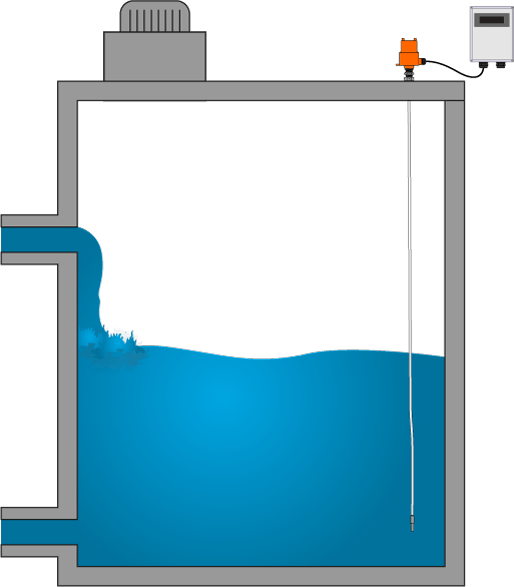
\includegraphics[width=0.6\textwidth]{img/tanque-de-vacuo-para-o-sistema-de-esgoto.png}
    \label{fig:tank}
\end{figure}

\newpage
\section{Objetivos}

Para auxiliar no planejamento de etapas do projeto, foram elencados e ordenados os objetivos principais para o projeto do sistema:
\begin{itemize}
    \item Avaliar a planta, com o objetivo de se familiarizar com o processo;
    \item Identificar e listar variáveis relevantes para o controle da planta;
    %\item Extrair parâmetros de interesse para a modelagem posterior;
    \item Desenvolver um modelo matemático;
    %preliminar
    que descreva o processo em malha aberta;
    \item Testar e validar a conexão do controlador com a planta;
    \item Desenvolver um controlador para regular o sistema; 
    \item Avaliar a eficiência do controlador através dos ensaios com o sistema;
    \item Selecionar o controlador mais adequado para o sistema;
    \item Desenvolver uma comunicação entre operador e planta;
    \item Desenvolver uma interface para operação do usuário do sistema.
    %\item Exportar os dados, obtidos em simulação, para um cliente externo;
    %\item Comparar os resultados obtidos nos dois itens anteriores.
\end{itemize}

\newpage


\section{Modelagem do Sistema em Malha Aberta}
\subsection{Metodologia}
% Programa em \textit{python} que controla a planta de forma a oter dados utilizados de forma a avaliar a sua resposta utilizando alguma ferramenta de análise de dados, para extrair o parâmetros para um modelo do sistema.

% \begin{center}
% \begin{tikzpicture}[auto, node distance=2cm,>=latex']
% \node [input, name=input] {};
%     \node [sum, right of=input] (sum1) {};
%     \node [sum, right of=sum1] (sum2) {};
%     \node [block, right of=sum2] (system) {G(s)};
%     \node [block, right of=system, node distance= 3cm] (controller) {\equation$\frac{1}{s}$};
%     \node [output, right of=controller] (output) {};
    
%     \node [block, below of=system] (feedback2) {$K_1$};
%     \node [block, below of=feedback2] (feedback1) {$K_2$};
    
%     \draw [draw,->] (input) -- node {$R(s)$} (sum1);
%     \draw [draw,->] (sum1) -- node {} (sum2);
%     \draw [draw,->] (sum2) -- node {} (system);
%     %\draw [->] (sum1) -- node {$e$} (controller);
%     \draw [->] (system) -- node [name=u] {} (controller);
%     \draw [->] (controller) -- node [name=y] {$Y(s)$} (output);
%     \draw [->] (u) |- (feedback2);
%     \draw [->] (feedback2) -| node[pos=0.99] {$-$} node {} (sum2);
%     \draw [->] (y) |- (feedback1);
%     \draw [->] (feedback1) -| node[pos=0.99] {$-$} node [near end] {$y_m$} (sum1);
% \end{tikzpicture}
% \end{center}

\subsubsection{Desenvolvimento da Planta Modelo}

Para simular o reservatório com as válvulas e sensores descritos na sessão \ref{ssec:intro}, foi utilizado o programa \factorio {} partindo de uma planta exemplo. O modelo em questão é uma planta de tanque atmosférico, controlada por um painel elétrico e com leitores de nível e fluxo.
 
 %figura planta Factoryio   
\begin{figure}[H]
    \centering
    \caption{Planta de simulação no Software \factorio{}}
    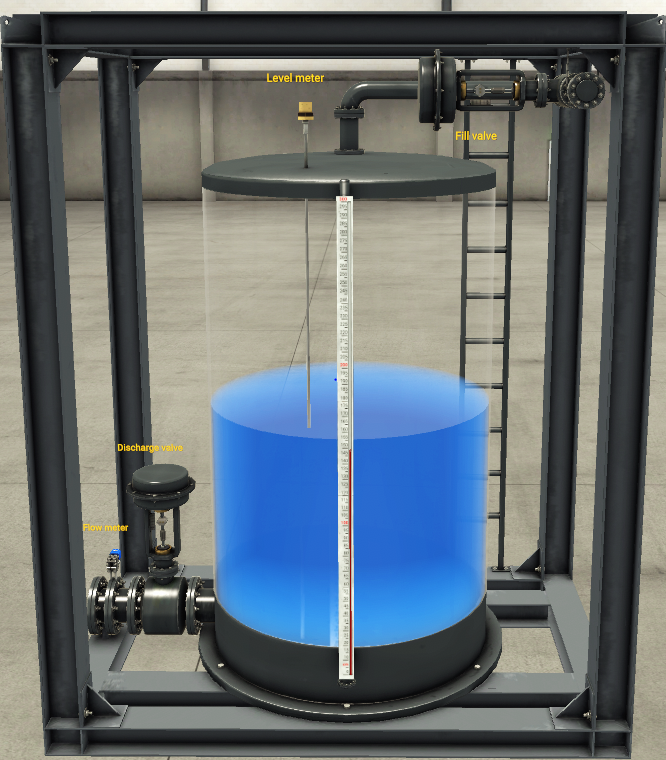
\includegraphics[width=0.5\textwidth]{img/factory IO.PNG}
    \label{fig:planta-factory-io}
\end{figure}
    
Com o modelo carregado, foi realizado um diagrama de blocos para regulagem manual das válvulas e visualização dos valores de fluxo e nível no \textit{Control.io} (figura \ref{fig:control-io}). Apesar de não usado para a extração dos dados, esse programa de controle simples permitiu um estudo inicial da planta, identificando por exemplo que o nível se estabiliza na metade da altura sempre que as duas válvulas estiverem com o mesmo valor.

 %figura control.io   
\begin{figure}[H]
    \centering
    \caption{Blocos de controle no Software Control.io}
    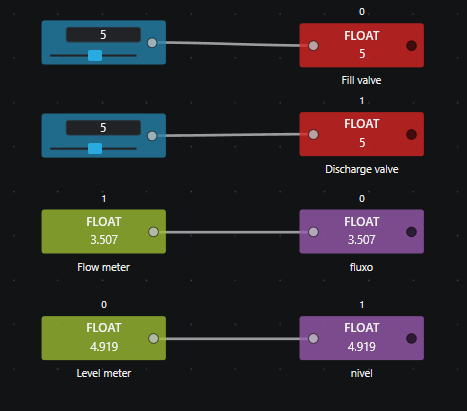
\includegraphics[width=.6\textwidth]{img/control io.PNG}
    \label{fig:control-io}
\end{figure}

\subsection{Obtenção de Dados}
\label{ssec:obt-dados}
De forma a obter dados, foi utilizada uma planta simulada na ferramenta \factorio, expondo seus atuadores por meio de um servidor \textit{Modbus} TCP (\textit{Transmission Control Protocol}). Este servidor foi controlado por um cliente escrito em \textit{python} e teve seus registradores conectados de maneira que pudesse controlar a simulação (fig. \ref{fig:conn-modbus}), os atuadores, e ler os sensores. 

\begin{figure}[H]
    \centering
    \caption{Diagrama de conexão do servidor Modbus}
    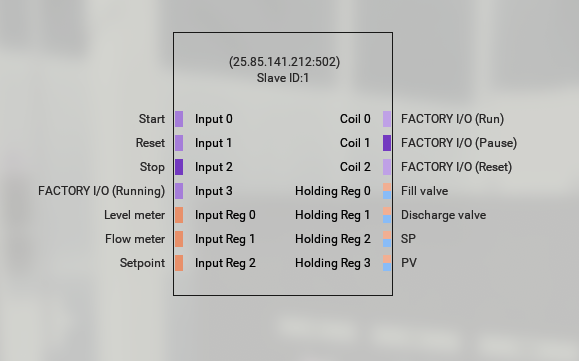
\includegraphics[width=\textwidth]{img/neg-factio-modbus-conn.png}
    \label{fig:conn-modbus}
\end{figure}

O cliente controla a planta de forma a estabelecer as condições iniciais para e realizar um teste de resposta a uma entrada de tipo \textit{step} unitário no sinal de controle da válvula de entrada à partir do equilíbrio ($h = 5m,~ v_{entrada}=v_{saida}=5.00$).

Os dados obtidos a partir deste teste foram exportados em formato CSV (\textit{Comma Separated Values}) e carregados no \textit{software} de análise matemática.

\subsubsection{Avaliação dos Dados}

Tomando os valores do experimento obtidos em \ref{ssec:obt-dados}, foi desenvolvida uma planilha para servir como banco de dados. Nessa planilha foram realizados os cálculos para obtenção dos modelos que descrevem a função, utilizando \texttt{query()},  fórmulas matemáticas e outras funções. O \textit{Google Sheets} foi a ferramenta adotada pois permite edição simultânea, organização na forma de banco de dados e conservação dos resultados de diversos experimentos. 

Os modelos matemáticos estudados foram:
\label{sec:metodo-modelos}
\begin{itemize}
    \item Ziegler/Nichols e Hägglund: Apesar de diferentes, ambos os métodos utilizam uma reta tangente traçada sobre o trecho de máxima inclinação, partindo do primeiro ponto de inflexão da curva e indo até o segundo, e portanto foram representados juntos aqui. Com a reta traçada, os parâmetros $t_1$, $t_2$ e $\theta$ são obtidos a partir do ponto de intersecção dela com o eixo t e do ponto em que o valor da função é igual ao valor máximo do experimento.
    
    \begin{minipage}{\linewidth}
        \centering
        \captionof{figure}{Exemplo da reta de Ziegler/Nichols}
        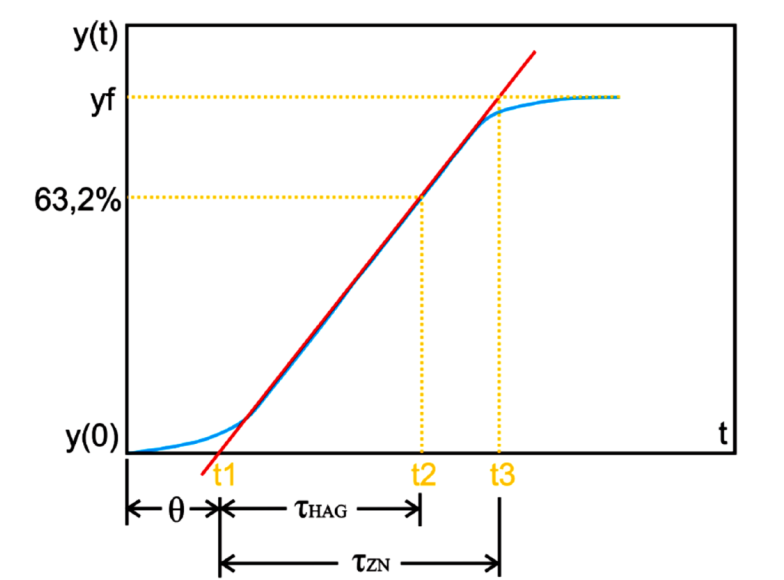
\includegraphics[width=0.5\textwidth]{img/ex-zn.png}
        \label{fig:ex-zn}
    \end{minipage}  
    
    Assim, como o caráter da resposta do sistema é sobreamortecido, ela não apresenta pontos de inflexão e esse modelo não pode ser aplicado.

    \item Smith: Diferente dos métodos de Ziegler/Nichols e Hägglund, este não utiliza o trecho de máxima inclinação para determinar os parâmetros necessários. Ao invés disso, utiliza-se os pontos correspondentes a 28.3\% e 63.2\% do valor máximo de saída, onde a curva costuma se aproximar muito de uma linearidade. 
    
    \begin{minipage}{\linewidth}
        \centering
        \captionof{figure}{Exemplo dos pontos de interesse para o método de Smith}
        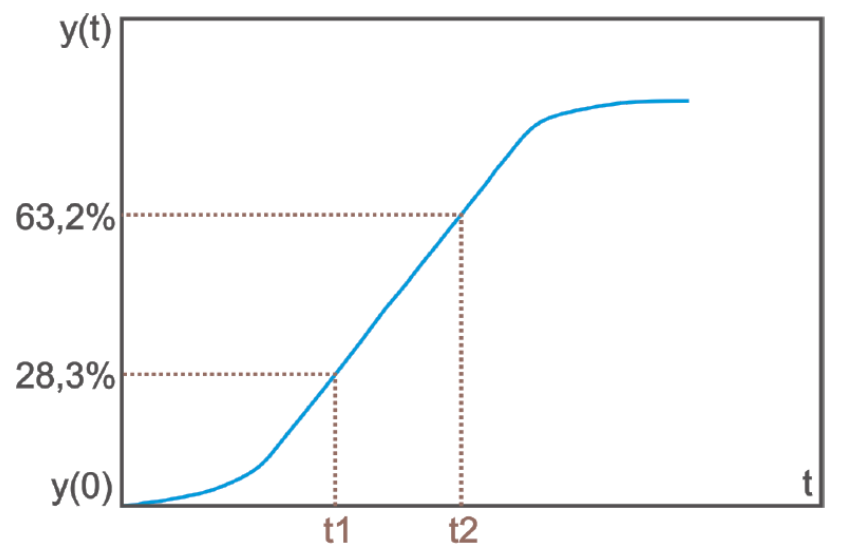
\includegraphics[width=0.5\textwidth]{img/ex-smith.png}
        \label{fig:ex-smith}
    \end{minipage}
    
    \item Sundaresan/Krishnaswamy: Semelhante ao método de Smith, também são definidos pontos onde a curva se aproxima da linearidade, porém nesse caso os pontos correspondem a 35.3\% e 85.3\% do valor máximo de saída.
    
    \begin{minipage}{\linewidth}
        \centering
        \captionof{figure}{Exemplo dos pontos de interesse para o método de Sundaresan/Krishnaswamy}
        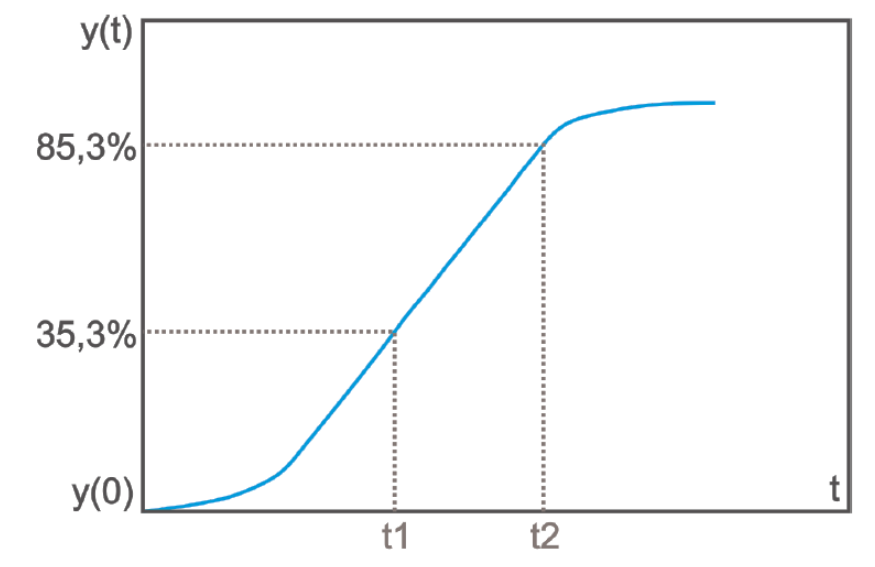
\includegraphics[width=0.5\textwidth]{img/ex-sundaresan.png}
        \label{fig:ex-sund}
    \end{minipage}
    
\end{itemize}


\subsubsection{Teste do Modelo Matemático}

Foi implementado um \textit{script} na ferramenta \textit{Matlab/Octave} para análise e comparação dos modelos obtidos com os dados da planta, que foram extraídos os dados da tabela de dados CSV. O resultado foi analisado a partir de um gráfico gerado usando a função \textit{step}, mostrando os comportamentos dos modelos e da planta.

\newpage
\subsection{Resultados Obtidos}
\subsubsection{Comportamento da Planta Simulada}

Para a análise do comportamento da planta, foi realizada uma simulação em um intervalo de 200 segundos. Nesse intervalo foi aplicado um sinal de entrada degrau, ou seja, o sinal da válvula de entrada mudou de 5 para 6.
% \begin{figure}[H]
%     \centering
%     \caption{Dados obtidos da planta}
%     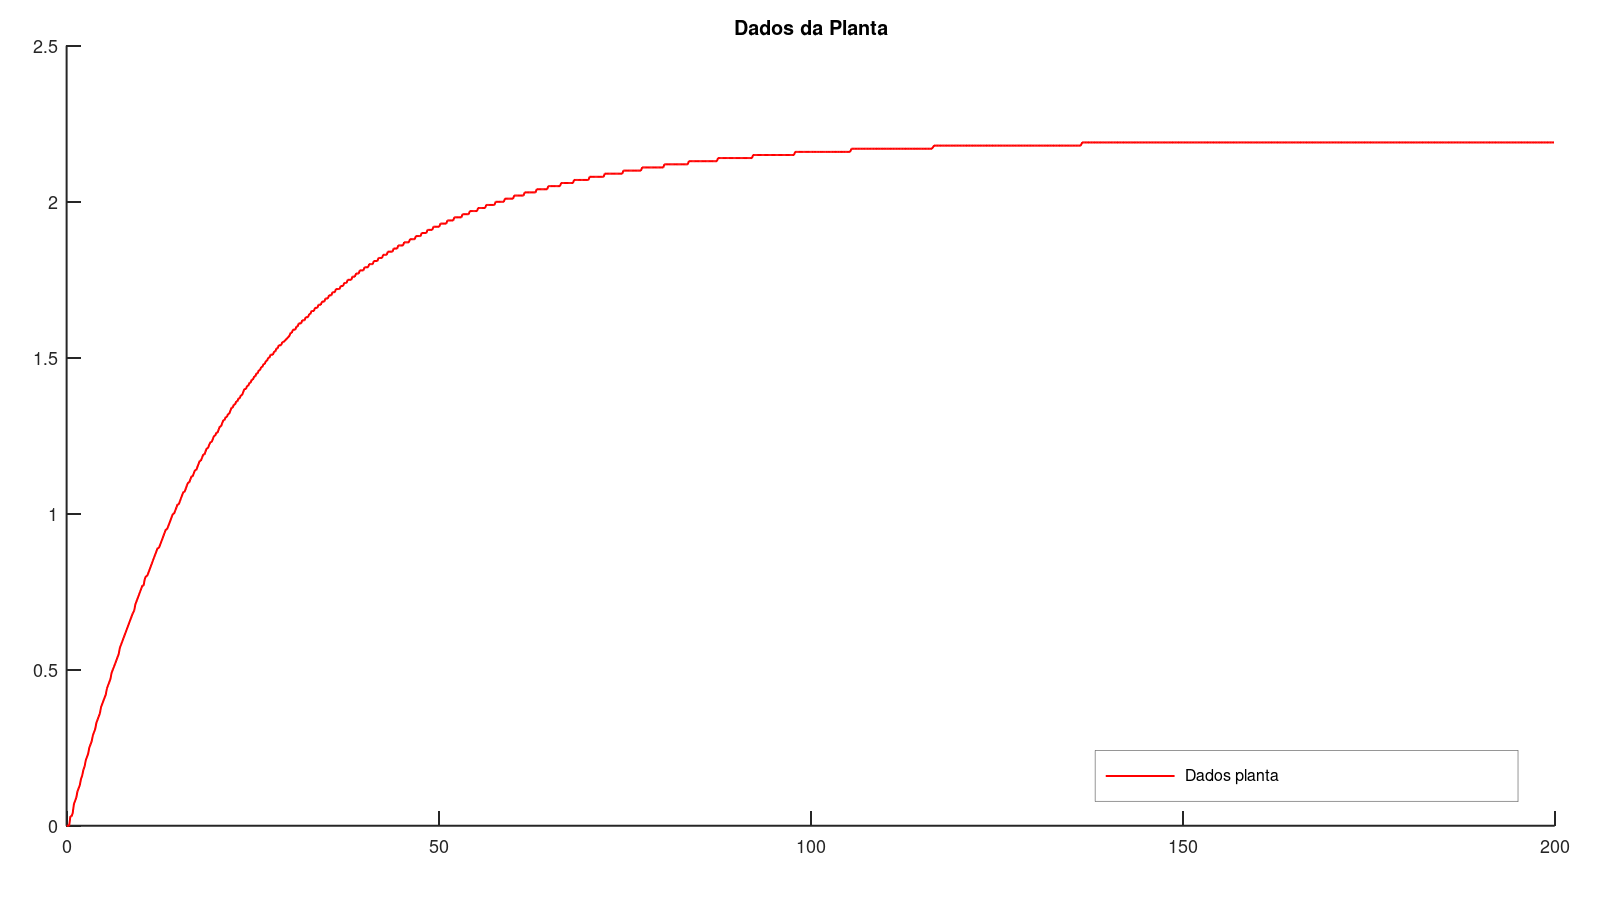
\includegraphics[width=0.8\textwidth]{img/dados-planta.png}
%     \label{fig:dados-planta}
%\end{figure}
\begin{figure}[H]
    \centering
    \caption{Dados Obtidos da planta}
    \begin{tikzpicture}
    \begin{axis}[xlabel=t (s),
                xmin = 0,
                ylabel=Nível (V),
                font=\small,
                width = \textwidth,
                height = 0.5\textwidth ]
    \addplot table [y=level, x=t, mark=none]{step_test.dat};
    %\addlegendentry{Resposta da planta}
    \end{axis}
    \end{tikzpicture}
    \label{fig:dados-planta}
\end{figure}

O gráfico apresentado na figura \ref{fig:dados-planta} representa o nível de água no tanque em função do tempo após o sinal aplicado na válvula de entrada. Como pode-se observar, a curva resultante do experimento apresenta um comportamento sobreamortecido, estabilizando o nível em 7V.

Além disso, algumas variáveis puderam ser obtidas, as quais estão destacadas na tabela \ref{tab:var-obtidas}:

\begin{table}[H]
    \centering
    \begin{tabular}{c|c|c}
        \toprule
        $\Delta$ Nível (V) & Tempo de Acomodação (s) & Tempo de Subida (s)\\
        \midrule
        2.19 & 91.120 & 55.310 \\
        \bottomrule
    \end{tabular}
    \caption{Variáveis Obtidas}
    \label{tab:var-obtidas}
\end{table}
% t_settle =  92.120

% descrever comportamento planta
\subsection{Obtenção dos Modelos Matemáticos}

Para a obtenção dos modelos, foram testados os dois métodos detalhados nos itens da seção \label{sec:metodo-modelos} que podem ser aplicados nesse sistema.
%Matlab para desenvolvimento do modelo matemático e octave
%Ajuste para adequação dos parametros
%\subsubsection{Ziegler/Nichols e Hägglund}
%Como descrito anteriormente, esses modelos usam uma reta tangente partindo dos pontos de inflexão para determinar os parâmetros. No entanto, dado o caráter da resposta do sistema (sobreamortecido), ela não apresenta pontos de inflexão e as tentativas de desenhar a reta se mostraram inconclusivas.

%Sendo assim, esses modelos foram descartados e foi dado seguimento na análise com os outros métodos, que não partem de uma reta tangente.

\subsubsection{Smith}
O método de Smith, também explicado anteriormente em \ref{sec:metodo-modelos}, foi o mais eficiente e preciso na comparação com o comportamento da planta. Assim, obteve-se os dados para a função de transferência, como $t_1$, $t_2$ $\tau$ e $\theta$:
\begin{equation}
\begin{split}
    t_1 = 7.94 s \\
    t_2 = 23.74 s \\
    \tau = 1.5* ( t_2 - t_1) = 23.70 \\
    \theta = t_2 - \tau = 0.04 \\
    G_p(s) = \frac{K_p e^{-\theta s}}{\tau s + 1} \\
    \theta \approx 0 \\
    G_p(s) = \frac{K_p}{\tau s + 1} \\
    G_p(s) = \frac{2.19}{23.7 s + 1} \\
\end{split}
\end{equation}

Como pode-se perceber, a variável $\theta$ (tempo de atraso) encontrada foi muito próxima de zero, podendo ser desprezada. Além disso, tendo em vista que esse termo representa o atraso da resposta, ele foi suprimido pois o teste com sinal de entrada degrau foi feito sem atraso.

\subsubsection{Sundaresan/Krishnaswamy}
Utilizando os métodos previamente descritos em \ref{sec:metodo-modelos}, a função obtida foi a exposta na equação \ref{eq:sundersan}, novamente ignorando o termo de atraso, como feito para o método de Smith. Assim, obteve-se os dados para a função de transferência, como $t_1$, $t_2$, $\tau$ e $\theta$:
\begin{equation}
\begin{split}
    t_1 = 10.5 s \\
    t_2 = 45.37 s \\
    \tau = 0.6* ( t_2 - t_1) = 20.922  \\
    \theta = 1.3*t_1 - 0.29*t2 = 0.4927 \\
    G_p(s) = \frac{K_p e^{-\theta s}}{\tau s + 1} \\
    \theta \approx 0 \\ 
    G_p(s) = \frac{K_p}{\tau s + 1} \\
    G_p(s) = \frac{2.19}{20.92 s + 1}
\end{split}
\label{eq:sundersan}
\end{equation}

\subsection{Comparação dos Modelos}
Após obtidos os modelos matemáticos simplificados, foi gerado um gráfico com as três curvas: Resultado do experimento, Modelo de Smith e Modelo de Sundaresan. 
% \begin{figure}[H]
%     \centering
%     \caption{Comparação dos modelos}
%     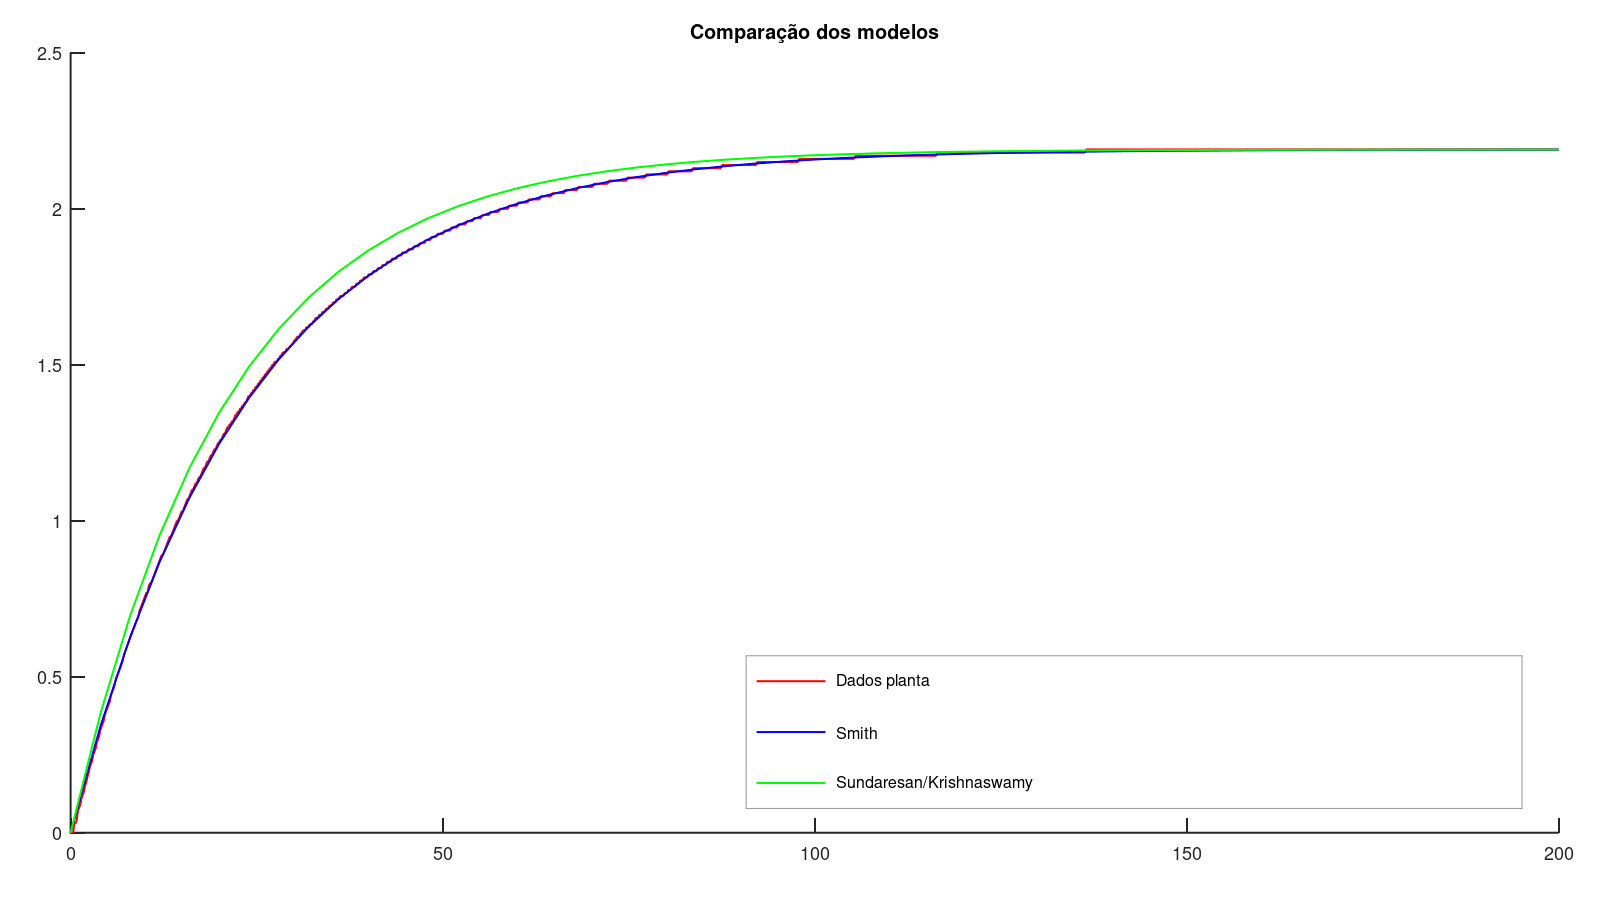
\includegraphics[width=0.8\textwidth]{img/comparacao-modelos.png}
%     \label{fig:comp-modelos}
% \end{figure}
\begin{figure}[H]
    \centering
    \caption{Comparação dos modelos}
    \begin{tikzpicture}
    \begin{axis}[xlabel=t (s),
                 xmin=0, xmax=220,
                 ymin=0,
                 ylabel=Nível (m),
                 legend pos=south east,
                 width = 0.95\textwidth,
                 height = 0.7\textwidth]
    \addplot[ultra thick, brown] table [y=Y_sund, x=T_sund, mark=none]{model_response.dat};
    \addlegendentry{Sundaresan}
    \addplot[ultra thick, red] table [y=y, x=t, mark=none]{step_test_norm.dat};
    \addlegendentry{Resposta da planta}
    \addplot[ultra thick, blue] table [y=Y_smith, x=T_smith, mark=none]{model_response.dat};
    \addlegendentry{Smith}
    \end{axis}
    \end{tikzpicture}
    \label{fig:comp-modelos-sund}
\end{figure}

Vale ressaltar que na figura \ref{fig:comp-modelos-sund}, as curvas de resposta da planta (em azul) e de Smith (em vermelho) estão visualmente sobrepostos, o que pode gerar confusão visual mas demonstra a acurácia do método no sistema aplicado.

A figura \ref{fig:comp-modelos-sund} mostra, em vermelho, a curva obtida pelo modelo de Smith, em cinza, o modelo de Sundaresan e, em azul, o resultado obtido na planta simulada. Destaca-se que as curvas atingem o mesmo valor de 2m de crescimento de nível no momento de estabilização e se comportam de forma semelhante.

Vale ressaltar que na figura \ref{fig:comp-modelos-sund} foi removido o valor médio de forma a obter uma visualização melhor. Além disso, os valores no eixo t vão desde o instante que é alterado o valor da válvula de entrada (estando no equilíbrio com $h=5m$) até a estabilização da planta.

Pode-se observar que o modelo de Smith é muito próximo dos dados do teste de entrada degrau, sendo que a maior parte da diferença advém de erro de quantização (Erro originado da precisão do sensor de nível), já que o sistema de leitura possui precisão de até 0.01 V.

Dessa forma, para as próximas etapas do projeto o ponto de partida será o modelo simplificado de Smith, descrito pela equação: 
\begin{equation}
     G(s) = \frac{2.19}{23.7 s + 1}
     \label{eq:planta}
\end{equation}
De modo a operar entre $0 \to 1$, o modelo normalizado da planta será o modelo obtido dividido por 10, pois o valor recebido pelo sensor para desenvolvimento da equação estava na faixa entre $0 \to 10$ V:
\begin{equation}
    G(s) = \frac{0.219}{23.7 s + 1}
\end{equation}
 
% descrever  diferenças entre modelos

%\subsection{Conclusão}
    %Reobservando os objetivos de estudar a planta, extrair os parâmetros fundamentais, desenvolver um modelo para equacionamento do sistema e exportar os dados. Pode-se dizer que o projeto cumpriu aquilo que foi estipulado até então, pois através dos dados extraídos com a planta simulada, o servidor \textit{modbus} e o modelo de equação desenvolvido, foi possível compreender o comportamento da planta e obter as informações necessárias para o desenvolvimento de um controlador PID.

	%Olhando para as próximas etapas do trabalho, ainda será acrescido a esse projeto um sistema de controle e um supervisório para operação da planta. Dessa forma, foram concluídas apenas as etapas de extração de dados e estudo do projeto.

\section{Modelagem do Controlador}
\subsection{Arquitetura de Comunicação}

% \begin{center}
% \begin{tikzpicture}[auto, node distance=2cm,>=latex]
    % \node [input, name=SP, node distance=3cm] {};
    % \node [sum, right of=SP] (sum) {};
    
    % \node [block, right of=sum] (controller) {Controlador};
    % \node [input, node distance=1.5cm, below of=controller] {Python};
    
    % \node [block, right of=controller, node distance=5cm] (sys) {Planta};
    
    % \node [block, right of=controller] (modbusin) {Modbus};
    % \node [block, right of=modbusin] (system) {Planta};
    % \node [output, right of=system] (output) {Nível};
    % \node [block, below of=modbusin] (modbusout) {Modbus};
    
    % \node [block, below of=system] (feedback2) {$K_1$};
    % \node [block, below of=feedback2] (feedback1) {$K_2$};
    
    % \draw [->] node {} (SP) -- node {Setpoint} (sum);
    % \draw [draw,->] (sum) -- node {} (controller);
    % \draw [->] (controller) -- node [name=u] {Sinal de controle} (modbusin);
    % \draw [->] (modbusin) -- node [u] {Sinal de controle} (system);
    % \draw [->] (output) -- node {$-$} (sum);
    % \draw [->] (sum) -- node {} (controller);
    % \draw [->] (input) -- node [] {+} (sum);
    % \draw [->] (output) -- node [name=y] (output);
    % \draw [->] (y) |- (sum);
    % \draw [->] (feedback2) -| node[pos=0.99] {$-$} node {} (sum2);
    % \draw [->] (y) |- (feedback1);
    % \draw [->] (feedback1) -| node[pos=0.99] {$-$} node [near end] {$y_m$} (sum1);
% \end{tikzpicture}
% \end{center}


\begin{figure}[H]
    \centering
    \caption{Layout orientado a comunicação}
    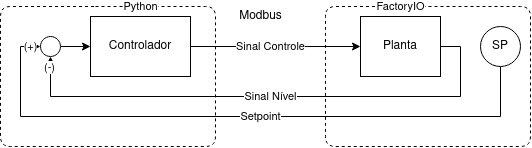
\includegraphics[width=\textwidth]{img/arq-comm.png}
    \label{fig:arq-comm}
\end{figure}

\subsection{Metodologia}
    Para obtermos a equação que rege o controlador, inicialmente foram feitos alguns modelos diferentes para que os resultados pudessem ser analisados. Assim, como de costume ao se projetar um controlador da família PID, começamos calculando e testando um controlador do tipo Proporcional e, em seguida, um controlador do tipo Proporcional-Integrador.
    
    Em cada caso, foi manipulada a equação \ref{eq:planta} de forma a incluir a ação do controlador em questão, inserindo os ganhos relevantes.
\subsubsection{Controlador P}
Tomando o controlador:
\begin{equation}
C(s) = K_p
\end{equation}

Em malha aberta:
\begin{equation}
    G_pa(s) = \frac{K_p \cdot 0.219}{23.7 \cdot s + 1}
     \label{eq:planta-com-p}
\end{equation}

Em malha fechada:

\begin{equation}
 G_p(s) = \frac{K_p \cdot 0.219}{23.7 \cdot s + (1 + K_p \cdot 0.219)}
\end{equation}

    Foi calculado um controlador Proporcional de forma a atender o requisito inicial de $E_{reg}$ de 10\%, utilizando a equação do próprio Erro de Regime:
    
    \begin{equation}
     E_{reg} = \lim_{s \to 0} s \cdot \left( U(s) - U(s) \cdot G_p(s) \right)
    \label{eq:e-reg}
    \end{equation}
    Sendo o sinal de entrada U(s) um sinal degrau, teremos:
    \begin{equation} \begin{split}
        E_{reg} = \lim_{s \to 0} s \cdot \left( \frac{1}{s} - \frac{1}{s} \cdot \frac{K_p \cdot 0.219}{23.7 \cdot s + (1 + K_p \cdot 0.219)} \right) \\
        E_{reg} = 1 -\frac{K_p \cdot 0.219}{(1 + K_p \cdot 0.219)} \\
        E_{reg} = 0.1 = 1 -\frac{K_p \cdot 0.219}{(1 + K_p \cdot 0.219)} \\
        0.9 = \frac{K_p \cdot 0.219}{(1 + K_p \cdot 0.219)} \\
        0.9 + K_p \cdot 0.9 \cdot 0.219 = K_p \cdot 0.219 \\
        0.9 = K_p \cdot  (0.219 - 0.9 \cdot 0.219) \\ 
        K_p = \frac{0.9}{0.1 \cdot 0.219} = 41.0959 \\
    \end{split} \label{eq:calc-e-reg} \end{equation}
        % E_{reg} = \lim_{s \to 0} \left( 1 - \frac{K_p \cdot 0.219}{23.7 \cdot s + (1 + K_p \cdot 0.219)} \right)\\
        % - 0.495 = \frac{0.1 - 0.9 \cdot 0.219 \cdot K_p}{1 + K_p\cdot 0.219} \\
        % - 0.495 \cdot (1 + K_p\cdot 0.219) = 0.1 - 0.9 \cdot 0.219 \cdot K_p \\
        % - 0.108405 \cdot K_p + 0.9 \cdot 0.219 \cdot K_p = 0.595 \\
        % K_p = \frac{0.595}{0.9 \cdot 0.219 - 0.108405} = 6.70838266\\
    
\subsubsection{Controlador PI}
 já em malha fechada
\begin{equation}
     G_p(s) = \frac{ ( K_p \cdot s + K_i) \cdot 0.219 }{23.7 \cdot s^2 + (1 + K_p \cdot 0.219) \cdot s  + K_i \cdot 0.219}
     \label{eq:planta-com-pi}
\end{equation}

    %Os ganhos foram calculados de forma a atender um sobressinal de 5\%, o que leva a 
    %$\xi = 0.69$.
    % Considerando a equação de $G(s)$ normalizada:
    % \begin{equation}
    %     G(s) = \frac{(K_p \cdot 0.219}{23.7 \cdot s + 1} \\
    % \end{equation}
    
    Comparando a equação de $G_p$ com a sua forma canônica, tendo como objetivo um sobressinal de 5\%, erro nulo e tempo de acomodação de 30s, ou seja $\xi = 0.69$ ($S_0 = 0.05$) e estimando $t_a = 30s$, temos que:
    \begin{equation} \begin{split}
        %\frac{1}
        s^2 + s \cdot 2 \cdot \xi \cdot \omega_n + \omega_n^2  \text{, e   } %\frac{K_p \cdot s + K_i} 
        23.7 \cdot s^2 + (1 + K_p \cdot 0,219) \cdot s + K_i \\
        t_a = \frac{4}{0.69 \cdot \omega_n} \\
        \omega_n = \frac{4}{0.69 \cdot t} \\
        \omega_n = 0.1159 \frac{rad}{s} \\
    \end{split} \end{equation}
    Encontrando $K_i$ : 
    \begin{equation} \begin{split}
        \frac{K_i \cdot 0.219}{23.7} = \omega_n^2 \\
        K_i = \omega_n^2 \cdot \left( \frac{23.7}{0.219} \right) = 1.453
    \end{split} \end{equation}
        Encontrando $K_p$ :
    \begin{equation} \begin{split}
        \frac{1 + K_p \cdot 0.219}{23.7} =  \omega_n \cdot \xi \\
        K_p =  \frac{23.7 \cdot 2 \cdot \omega_n \cdot \xi - 1}{0.219} = 12.7426 
    \end{split} \end{equation}

\subsubsection{Controlador PID}
 já em malha fechada
\begin{equation}
     G_p(s) = \frac{ (K_d \cdot s^2 + K_p \cdot s + K_i) \cdot 0.219 }{(23.7 + 0.219 \cdot K_d) \cdot s^2 + (1 + K_p \cdot 0.219) \cdot s  + K_i \cdot 0.219}
     \label{eq:planta-com-pi}
\end{equation}

    %Os ganhos foram calculados de forma a atender um sobressinal de 5\%, o que leva a 
    %$\xi = 0.69$.
    % Considerando a equação de $G(s)$ normalizada:
    % \begin{equation}
    %     G(s) = \frac{(K_p \cdot 0.219}{23.7 \cdot s + 1} \\
    % \end{equation}
    
    Comparando a equação de $G_p$ com a sua forma canônica, tendo como objetivo um sobressinal de 5\%, erro nulo e tempo de acomodação de 30s, ou seja $\xi = 0.69$ ($S_0 = 0.05$) e estimando $t_a = 30s$, temos que:
    \begin{equation} \begin{split}
        %\frac{1}
        s^2 + s \cdot 2 \cdot \xi \cdot \omega_n + \omega_n^2  \text{, e   } %\frac{K_p \cdot s + K_i} 
        (23.7 + 0.219 \cdot K_d) \cdot s^2 + (1 + K_p \cdot 0.219) \cdot s  + K_i \cdot 0.219 \\
        t_a = \frac{4}{0.69 \cdot \omega_n} \\
        \omega_n = \frac{4}{0.69 \cdot t} \\
        \omega_n = 0.1159 \frac{rad}{s} \\
    \end{split} \end{equation}
    Encontrando $K_i$ : 
    \begin{equation} \begin{split}
        \frac{K_i \cdot 0.219}{0,219 \cdot k_d + 23.7} = \omega_n^2 \\
        K_i = \omega_n^2 \cdot \left( \frac{0,219 \cdot k_d + 23.7}{0.219} \right)
    \end{split} \end{equation}
        Encontrando $K_p$ :
    \begin{equation} \begin{split}
        \frac{1 + K_p \cdot 0.219}{23.7 + K_d \cdot 0.219} = 2 \cdot \omega_n \cdot \xi \\
        K_p =  \frac{2 \cdot \xi \cdot \omega \cdot (23.7 + K_d \cdot 0.219) - 0.219}{0.219} \\
    \end{split} \end{equation}
    
Supondo $K_d = 5$ nas equações anteriores, temos $K_i = 1,517$ e $K_p = 13,539$.
%Apenas em caráter experimental, foram tomados como base os ganhos do controlador PI e, em conjunto de um pequeno $K_d = 0.5$, foi aplicado um controle PID completo para avaliar a resposta obtida.
\subsubsection{Modelagem Discreta Direta}
Com o objetivo de prova para o método direto do cálculo dos ganhos no modelo discreto, foi calculado um controlador P para a planta no domínio Z, usando apenas um requisito, de tempo de acomodação ($t_a$) de 40 segundos. Sendo a planta:
\begin{equation}
   G(s) = \frac{0.219}{23.7 s + 1} 
\end{equation}

Começamos encontrando a equação da planta no domínio Z, utilizando a transformada de $\frac{G(s)}{s}$ e o segurador de ordem zero:

\begin{equation} 
\begin{split}
    G(z) = (1-z^{-1}) \cdot \mathcal{Z} \left\{ \left. \left( \mathcal{L} \left\{ \frac{G(s)}{s} \right\} \right) \right| _{t=kT} \right\} \\
    G(z) = (1-z^{-1}) \cdot \mathcal{Z} \left\{ \left. \left( \mathcal{L} \left\{ \frac{0.219}{s(23.7 s + 1)} \right| _{t=kT} \right\} \right)  \right\} \\
\end{split}
\end{equation}

Utilizando a identidade:
\[ \frac{a}{s(s+a)} = \frac{1-e^{-aT} z^{-1}}{(1 - z^{-1})\cdot(1-e^{-at}z^{-1})} \]

\begin{equation} 
    G(z) = 0.219 \cdot \frac{(1-e^{-\frac{T}{23.7}})z^{-1}}{1-e^{-\frac{T}{23.7}}z^{-1}}
\end{equation}
%          c = e^{-\frac{T}{23.7}}
Multiplicando por $\frac{z}{z}$ para levar a equação a valores positivos nos expoentes de z:
\begin{equation} 
    G(z) =  \frac{0.219(1-e^{-\frac{T}{23.7}})} {z-e^{-\frac{T}{23.7}}}
\end{equation}
Para o requisito apresentado, teremos os polos em S da seguinte forma: (para tempo de acomodação de 98\%)

\begin{equation}
\begin{split}
    t_a=40s \\
    t_a=\frac{4}{|polo|} \\
    Polo = 0.1 \\
    S = -0.1 \\
\end{split}
\end{equation}

Desse polo em S, transformamos em polo de Z pelo método abaixo, e em seguida montamos a equação do polinômio característico que procuramos: ($T=0.3$)
\begin{equation}
\begin{split}
    Z=e^{sT}=0.97 \\
    F_d(z)=z-0.97 \\
\end{split}
\end{equation}
Agora, para a equação do controlador em si, assumiremos seu grau como 1, já que o grau da planta também ficou em 1. Assim:
\begin{equation}
\begin{split}
    C(z)=\frac{K(z+c_1)}{(z+c_2)} \\
    F_t(z)=G(z) \cdot C(z) \\
    F_t(z)=\frac{K(z+c_1)}{(z+c_2)} \cdot \frac{0.219(1-e^{-\frac{T}{23.7}})} {z-e^{-\frac{T}{23.7}}} \\
\end{split}
\end{equation}

Agora, para reduzir a quantidade de variáveis livres, definimos $c_1=e^{-\frac{T}{23.7}}$, obtendo assim a equação para $F_t(z)$, que então usamos para fechar a malha:
\begin{equation}
\begin{split}
    F_t(z)=\frac{0.219K(1-e^{-\frac{T}{23.7}})}{(z+c_2)} \\
    \frac{Y(z)}{R(z)}=\frac{F_t(z)}{1-F_t(z)} \\
    \frac{Y(z)}{R(z)}=\frac{0.219K(1-e^{-\frac{T}{23.7}})}{0.219K(1-e^{-\frac{T}{23.7}})+(z+c_2)} \\
\end{split}
\end{equation}
Comparando o divisor da equação com o polinômio característico que encontramos anteriormente, chegamos a uma equação que relaciona K com $c_2$, ambos desconhecidos:
\begin{equation}
\begin{split}
   0.219K(1-e^{-\frac{T}{23.7}})+(z+c_2) = (z-0.97) \\
   c_2=-0.97-0.002755K \\
\end{split}
\end{equation}
Utilizamos alguns testes para definir os valores de $c_2$ e K e, assim, podermos chegar a equação final para o controlador, e realizar testes com os resultados encontrados aqui.
\begin{equation}
\begin{split}
   C(z)=\frac{K(z-0.98742)}{z+c_2}
\end{split}
\end{equation}
\begin{equation}
\begin{split}
     K= 10.95 ; c_2= -1.0002
\end{split}
\end{equation}
A partir disso, combinou-se a equação do controlador (27) com a equação (25) da função transferência e o modelo foi testado no \textit{MatLab}, obtendo a seguinte curva resposta:
\begin{figure}[H]
    \centering
    \caption{Simulação no \textit{Matlab} com controlador discreto}
    %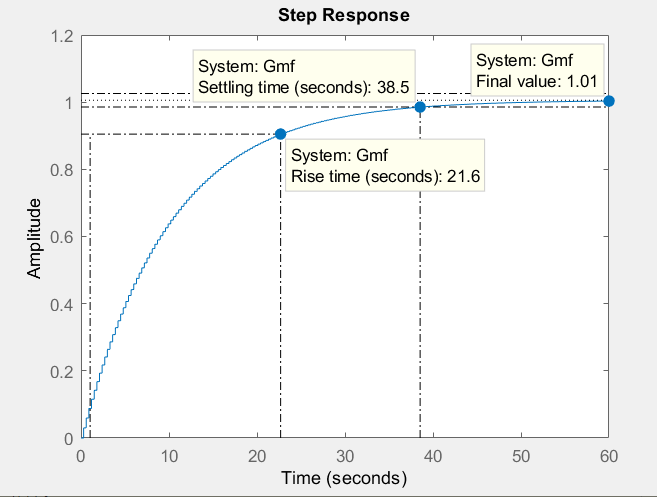
\includegraphics[width=\textwidth]{img/grafico discreto.png}
    \begin{tikzpicture}
    \begin{axis}[xlabel=t (s),
               xmin = 0, xmax=,
               ymin = 0, ymax = 1.2,
               ylabel=Amplitude,
               font=\small,
               width = \textwidth,
               height = 0.5\textwidth ]
    \addplot table [y=t, x=A, mark=none]{res.dat};
    \addlegendentry{Resposta com controlador discreto}
    \end{axis}
    \end{tikzpicture}
    \label{fig:res-discreto}
    \end{figure}
    
Com a curva, ficou comprovado que o sistema atendeu o requisito de tempo de acomodação, estabilizando 2s antes do estipulado. 
\subsection{Resultados Obtidos}
\subsubsection{Controlador P}
Inserindo o controlador do tipo proporcional no sistema em malha fechada, tomando como expectativa o erro assumido de 1\% e aplicando o ganho calculado $K_p = 99$, obteve-se a seguinte resposta na simulação:

\begin{figure}[H]
    \centering
    \caption{Teste P}
    \begin{tikzpicture}
    \begin{axis}[
    xlabel=t (s),
    xmin=0, xmax=\xPID,
    ymin=-0.15, ymax=\yPID,
    font=\small,
    %ylabel=Nível (m),
    legend pos=north east,
    width = 0.95\textwidth,
    height = 0.7\textwidth]
    \addplot[brown] table [y=out_valve, x=t, mark=none]{teste-P.csv};
    \addlegendentry{Sinal de controle}
    \addplot[red] table [y=level, x=t, mark=none]{teste-P.csv};
    \addlegendentry{Nível no tanque}
    \addplot[green] table [y=setpoint, x=t, mark=none]{teste-P.csv};
    \addlegendentry{Setpoint}
    \addplot[blue] table [y=error, x=t, mark=none]{teste-P.csv};
    \addlegendentry{Erro}
    \end{axis}
    \end{tikzpicture}
    \label{fig:comp-modelos-P}
\end{figure}

Como pode-se observar, ao atingir o valor pré-definido, o nível fica oscilando com um erro máximo de 1.8\% e como o controle é apenas proporcional, o sinal de controle oscila excessivamente, entre o seu valor máximo e mínimo. Isto seria altamente danoso à um equipamento real e geraria grande desgaste, o que tornaria este controle impraticável. Uma solução mais adequada neste caso, seria utilizar um controle ON/OFF com histerese. 

%isso porque o sinal de controle é completamente instável e não apresenta perspectiva de estabilização em nenhum momento, sendo essa uma característica esperada em controladores P nesse cenário. Ou seja, apesar do sistema se aproximar do requisito de erro estipulado, ele se torna impraticável.

\subsubsection{Controlador PI}
Inserindo o controlador do tipo Proporcional-Integrativo no sistema em malha fechada, sabendo que um controlador PI apresenta erro de 0\% e tomando como expectativa um sobressinal assumido de 5\%, aplicando os ganhos calculados $K_p = 12.6455$ e $K_i = 3.4394$ resultou na seguinte resposta de simulação:

\begin{figure}[H]
    \centering
    \caption{Teste PI}
    \begin{tikzpicture}
    \begin{axis}[xlabel=t (s),
                 xmin=0, xmax=\xPID,
                 ymin=-0.15, ymax=\yPID,
                 ylabel=Valores normalizados,
                 legend pos=north east,
                 font=\small,
                 width = 0.95\textwidth,
                 height = 0.7\textwidth]
    \addplot[blue] table [y=error, x=t, mark=none]{teste-PI.csv};
    \addlegendentry{Erro}
    \addplot[red] table [y=level, x=t, mark=none]{teste-PI.csv};
    \addlegendentry{Nível do tanque}
    \addplot[green] table [y=setpoint, x=t, mark=none]{teste-PI.csv};
    \addlegendentry{Setpoint}
    \addplot[brown] table [y=out_valve, x=t, ]{teste-PI.csv};
    \addlegendentry{Sinal de controle}
    \end{axis}
    \end{tikzpicture}
    \label{fig:comp-modelos-PI}
\end{figure}

Como esperado em um controlador PI, o erro em regime é nulo. Além disso, o sobressinal máximo obtido foi de 1.45\%, ou seja, muito abaixo dos 5\% esperados, fazendo com que o nível no tanque ultrapasse muito pouco o valor desejado antes de estabilizar. Já o tempo de acomodação é de 35s, excedendo o valor estipulado, mas ainda sendo útil em um sistema real.
    
\subsubsection{Controlador PID}

\begin{figure}[H]
    \centering
    \caption{Teste PID}
    \begin{tikzpicture}
    \begin{axis}[xlabel=t (s),
                 xmin=0, xmax=\xPID,
                 ymin=-0.15, ymax=\yPID,
                 %ylabel=Nível (m),
                 legend pos=north east,
                 font=\small,
                 width = 0.95\textwidth,
                 height = 0.7\textwidth]
    \addlegendentry{Nível no tanque}
    \addplot[blue] table [y=error, x=t, mark=none]{teste-PID.csv};
    \addlegendentry{Setpoint}
    \addplot[red] table [y=level, x=t, mark=none]{teste-PID.csv};
    \addlegendentry{Erro}
    \addplot[green] table [y=setpoint, x=t, mark=none]{teste-PID.csv};
    \addlegendentry{Sinal de controle}
    \addplot[brown] table [y=out_valve, x=t, ]{teste-PID.csv};
    \end{axis}
    \end{tikzpicture}
    \label{fig:comp-modelos-PID}
\end{figure}

    Em caráter experimental, foi feito um teste com $K_d = 5$, utilizando os valores calculados na parte de metodologia. A resposta obtida foi um pouco mais oscilatória, mas sem nenhuma alteração significativa no valor de sobressinal (pelo menos no fundo de escala utilizado). No entanto, considerando o custo de implementação e a natureza do sistema este controlador não aparentou melhorias significativas.
    %Foram pesquisadas bibliotecas para a linguagem de programação utilizada no software de captura de dados, já tendo em mente a integração com o sistema de controle.
    %A biblioteca que será utilizada para a implementação inicial será a \href{https://pypi.org/project/simple-pid/}{Simple PID}. Será futuramente avaliada sua performance e precisão para a aplicação e se for necessário é sujeita a troca.
    %Essa etapa do projeto terá como ponto de partida o modelo matemático escolhido, além das restrições para determinação de um modelo de controle PID.
\newpage

\section{Integração de Sistemas}

\begin{figure}[H]
    \centering
\caption{\textit{Layout} de Comunicação Geral}
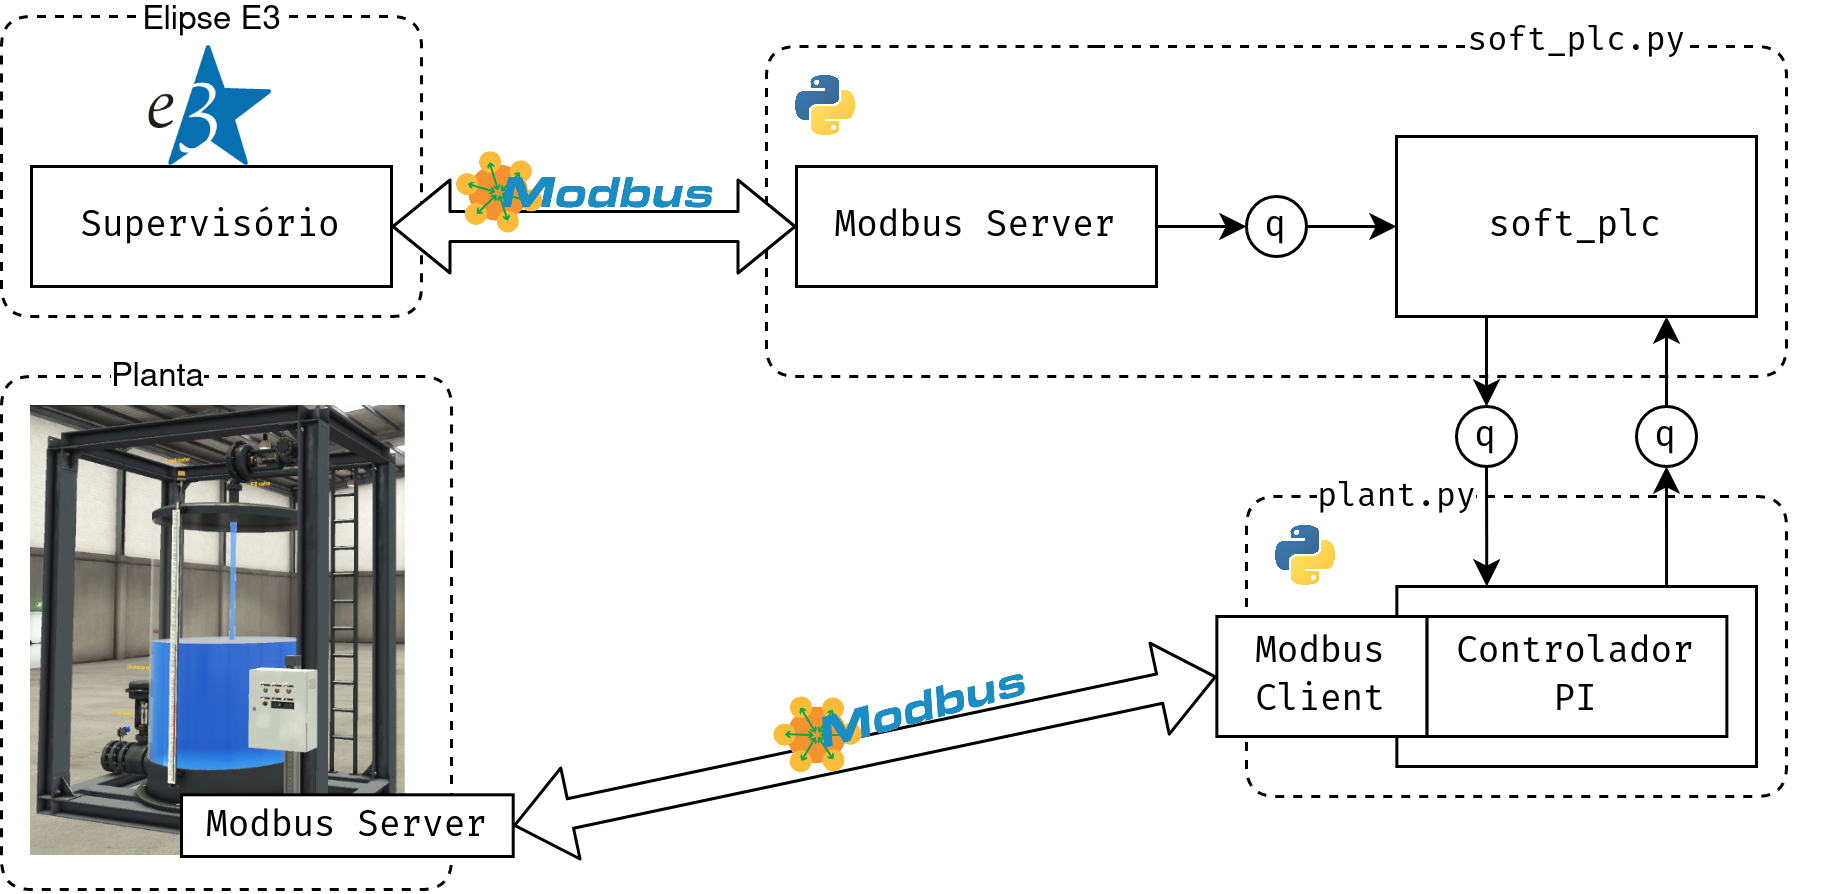
\includegraphics[width=0.8\textwidth]{img/diagrama-geral.png}
    \label{fig:arq_geral}
\end{figure}

Ao integrar o supervisório, o controlador e a planta, foram implementados 2 pares cliente-servidor \Mb: um entre o supervisório e o controlador, e outro entre o controlador e a planta; sendo um cliente e um servidor implementados em \Py.

Foram definidos registradores de entrada e saída para ambos os pares, sendo os da planta expostos na figura \ref{fig:conn-modbus} e do supervisório na figura \ref{fig:tags-comm-2}. 

Internamente na implementação em \Py, são utilizadas duas \textit{threads} que se comunicam via filas, representado no diagrama pela letra "\texttt{q}". Isto é feito de modo a desacoplar o tempo de execução dos dois processos. Além disso, essa é a forma recomendada de implementar comunicação e troca de dados segura entre processos sem problemas de concorrência e sincronismo (compartilhar memória é contraindicado e, na linguagem escolhida, praticamente impossível).

Por exemplo: o processo da planta, idealmente, deve rodar em um \textit{loop} de tempo fixo igual ao tempo de amostragem escolhido para o sistema (neste caso $T=0.3$). Integrar os dois componentes mantendo este requisito seria dispendioso e reduziria muito a modularidade do código.

A seguir serão abordadas as alternativas de comunicação testadas ao longo do projeto e, de uma forma mais detalhada, explicada como as partes do sistema interagem ao longo da execução.
%de registradores, dos quais são usados dois para realizar as operações de leitura e escrita das informações do servidor. O código do servidor assíncrono foi feito em \textit{Python} usando inicialmente a biblioteca \textit{PyModbus}.
%expando isso?
%Pode-se ver na figura \ref{fig:arq_geral} uma visão geral da arquitetura e a relação entre os componentes do sistema.

\subsection{Alternativas de \textit{Driver} e Comunicação}

Ao longo desse desenvolvimento, foram testadas diversas soluções para a troca de informações do supervisório com o servidor e outros elementos do sistema, visando uma que fosse funcional, estável e permitisse o envio e recebimento das informações precisas. Dessa forma, as principais alternativas consideradas estão listadas nos tópicos abaixo:

\begin{itemize}
    \item OPC/UA: foi utilizado para testes, no entanto não foi explorado pois mostrou-se demasiadamente complexo para a aplicação em questão.
    \item MQTT: apesar de possuir configuração e utilização bastante simples, o \textit{driver} deste protocolo disponível para \EE não permite, por algum defeito pontual, se conectar à rede quando a interface está operando. %possui um defeito onde conectava com sucesso se ligado manualmente, mas não quando ligado à interface.
    %F for MQTT ;-;
    %F -Wolf -ternao
    %éfi
    \item \Mb: 
    \begin{itemize}
        \item \EE~ - Foram testados dois \textit{drivers} cliente: \textit{Enron} e \textit{Modicon}; somente o \textit{driver} \textit{Modicon} funcionou corretamente, portanto foi o selecionado para utilização na solução final.
        \item Servidor \Py~ - Foram testadas duas bibliotecas que implementam servidores \Mb: \textit{PyModbus} e \textit{pyModbusTCP}; O driver \textit{PyModbus} foi escolhido por ser mais robusto e estar mais estável, visto que o \textit{PyModbusTCP} ainda está em versão preliminar.
        \end{itemize}
\end{itemize}

\subsection{Detalhamento da Solução Final}
Depois de definidas as alternativas de desenvolvimento escolhidas anteriormente, foi implementado um servidor usando a biblioteca \textit{PyModbus}. Nesse sistema, para cada evento ou escrita nos registradores, o servidor \Mb{} chama um \textit{callback}, ou processador do evento.

Cada um desses eventos, os quais contêm um código de função, endereço e valor, são colocados em uma fila e mapeados em comandos no processo \texttt{soft\_plc}, por meio de um dicionário onde a chave é o endereço onde ocorreu uma escrita e o valor é o comando associado. Abaixo está detalhado o código em questão.

%função processadora de evento, para o evento de qualquer escrita em registradores \Mb, estes eventos, cada um contendo um código de função, endereço e valor, são colocados em uma fila e mapeado em comandos no processo \texttt{soft\_plc}, por meio de um dicionário onde a chave o \texttt{dict} abaixo

\begin{minted}{python}
plant_co_map = {
    self.co.START_BTN.value: plant.Command.START,
    self.co.STOP_BTN.value:  plant.Command.STOP,
    self.co.EMERG_BTN.value: plant.Command.EMERGENCY,
    self.co.AUTO_MODE.value: plant.Command.AUTO_MODE,
}
plant_hr_map = {
    self.hr.IN_VALVE.value:  plant.Command.IN_VALVE,
    self.hr.OUT_VALVE.value: plant.Command.OUT_VALVE,
    self.hr.SETPOINT.value:  plant.Command.SETPOINT,
    self.hr.K_P.value:       plant.Command.SET_K_P,
    self.hr.K_I.value:       plant.Command.SET_K_I,
    self.hr.K_D.value:       plant.Command.SET_K_D,
}
\end{minted}
A cada ciclo de execução o processo \texttt{plant} lê valores da planta, via cliente \Mb, calcula o sinal de controle (se o controlador estiver habilitado) e gera resultados por meio de uma fila de saída, no formato especificado abaixo:

\begin{minted}{python}
res = {
    self.Output.TIME : 0,
    self.Output.LEVEL : 0,
    self.Output.OUTFLOW : 0,
    self.Output.OUT_VALVE : 0,
    self.Output.IN_VALVE : 0,
    self.Output.SETPOINT : 0,
    self.Output.DT : 0,
}
\end{minted}
Este ciclo é pensado de modo que, na medida do possível, haja um tempo de execução fixo (o principal limitador é o atraso da rede).

%No caso desses resultados comandos a serem enviados pelo controlador, estes são processados. O objeto de resultado têm a forma:

%Quanto ao processo da planta, a cada ciclo são produzidos objetos de resultado por meio de uma fila de saída e, no caso de comandos serem enviados pelo controlador, estes são processados. O objeto de resultado têm a forma:

Também, durante um ciclo, o processo checa se há itens na sua fila de entrada (cada item é um par de comando e valor), sendo que cada função obtida por este mapeamento é chamada com o valor associado. O mapeamento está exposto na seção de código abaixo:

\begin{minted}{python}
cmd_map = {
	self.Command.STOP : self.stop ,
	self.Command.START : self.start ,
	self.Command.EMERGENCY : self.emergency ,
	self.Command.AUTO_MODE : self.pid.set_auto_mode ,
	self.Command.SETPOINT : self.set_setpoint ,
	self.Command.IN_VALVE : self.set_in_valve ,
	self.Command.OUT_VALVE : self.set_out_valve ,
	self.Command.SET_K_P : self.set_kp ,
	self.Command.SET_K_I : self.set_ki ,
	self.Command.SET_K_D : self.set_kd ,
}
\end{minted}

Já no \texttt{soft\_plc}, os valores lidos da fila de saída de \texttt{plant} são utilizados para atualizar os endereços correspondentes à estes valores no servidor \Mb{}. Como a implementação \Mb{} utiliza somente números inteiros, todos os valores comunicados por meio de \Mb{} (desde a planta) possuem \textit{offset} decimal de 1000. Esta constante é informada ao supervisório por meio de um registrador. 

Sendo assim, os dados estão no formato adequado para serem compreendidos pelo \textit{driver} do supervisório e, consequentemente, pelo usuário.
%outro

\section{Supervisório}
\subsection{Estrutura do Supervisório}
%% O supervisório foi estruturado a partir de 3 classes: Elementos, Botões e Comunicação %%
Para desenvolvimento da interface para o usuário, foi feito um supervisório no \EE, o qual está estruturado com base em dois tipos de elementos, os atuadores e mostradores, conforme descrito abaixo.
 
\begin{itemize}
\item Atuadores
\begin{itemize}
    \item Botão de ligar: inicia o sistema, começando já ativado ao ligar o supervisório;
    \item Botão de parar: encerra a simulação no programa \factorio;
    \item Botão de emergência: fecha as válvulas e interrompe os sistemas imediatamente; 
    \item Carregar: atualiza valores de entrada de Kp, Ki, Kd e nível;
    \item Atualizar: atualiza a tabela referente; 
    \item Botões de Modo: alteram o modo de operação do sistema, de automático para manual;
    \item Abertura das válvulas de entrada e saída: alteram, através de um conjunto de controles deslizantes, a porcentagem de abertura das válvulas de entrada e saída;
    \item Salvar: atualiza a habilitação dos limites do alarme de nível e também seus respectivos valores;
    \item \textit{Login}: permite que o usuário realize \textit{login} no sistema;
    \item Análise gráfica: mostra um gráfico, em janela separada, com o comportamento do sistema ao longo do tempo;
    \item Configuração do sistema: abre uma janela modal onde se permite configurar parâmetros do sistema;
    \item Alarmes: abre uma janela modal onde se permite configurar o alarme de nível e também possui uma tabela com o histórico de disparos;
    \item Histórico de configurações: abre uma janela modal que possui tabelas demonstrando o histórico de alterações de parâmetros e também o histórico de valores do sistema.
\end{itemize}
\item Mostradores
\begin{itemize}
    \item Sinaleira: 3 luzes indicando o estado do sistema: funcionando, parado ou emergência;
    \item Nível: apresenta o nível atual de água no tanque, em metros e em \%;
    \item Fluxo: apresenta a taxa de passagem de fluido, em \%;
    \item Abertura das válvulas de entrada e de saída: mostra, em \%, o quão aberta está cada válvula;
    \item Erro: Expõe o erro, em \%, da resposta;
    \item Risco de nível: apresenta ao usuário a situação do nível do tanque de acordo com os limites do alarme;
    \item Ganhos: mostram os ganhos, Kp, Ki e Kd, atuais;
    \item Gráfico: registra o comportamento do sistema ao longo do tempo;
    \item Nível desejado: apresenta o valor de nível desejado mais recente estabelecido pelo usuário;
    \item Histórico de alarmes: tabela contendo os últimos alarmes de nível disparados e o usuário que os configurou;
    \item Histórico de configurações: tabela que armazena todas as alterações realizadas na configuração do sistema e o usuário responsável por elas;
    \item Histórico de dados da planta: tabela com a finalidade de apresentar um histórico de valores essenciais do sistema, atualizando-os a cada 5 segundos;
\end{itemize}
\end{itemize}

Nas próximas seções serão expostos como os elementos estão distribuídos nas telas e como ocorre a comunicação com a planta.

\subsection{Telas da Interface}

O supervisório é composto por cinco telas, onde a primeira é o Painel de Monitoramento. A sua principal função é apresentar a situação atual do sistema, contendo a sinaleira, os mostradores de nível, de fluxo, de erro e do estado das válvulas. Além disso, ela também têm os comandos básicos para iniciar, parar, acessar o gráfico do sistema, o painel de configuração do sistema e o painel de configuração dos alarmes. 

Além disso, possui um mostrador de alarme referente ao nível atual do tanque e seu risco potencial, bem como um botão de emergência, responsável por fechar ambas as válvulas o mais rápido possível.

\begin{figure}[H]
    \centering
    \caption{Tela de Monitoramento} 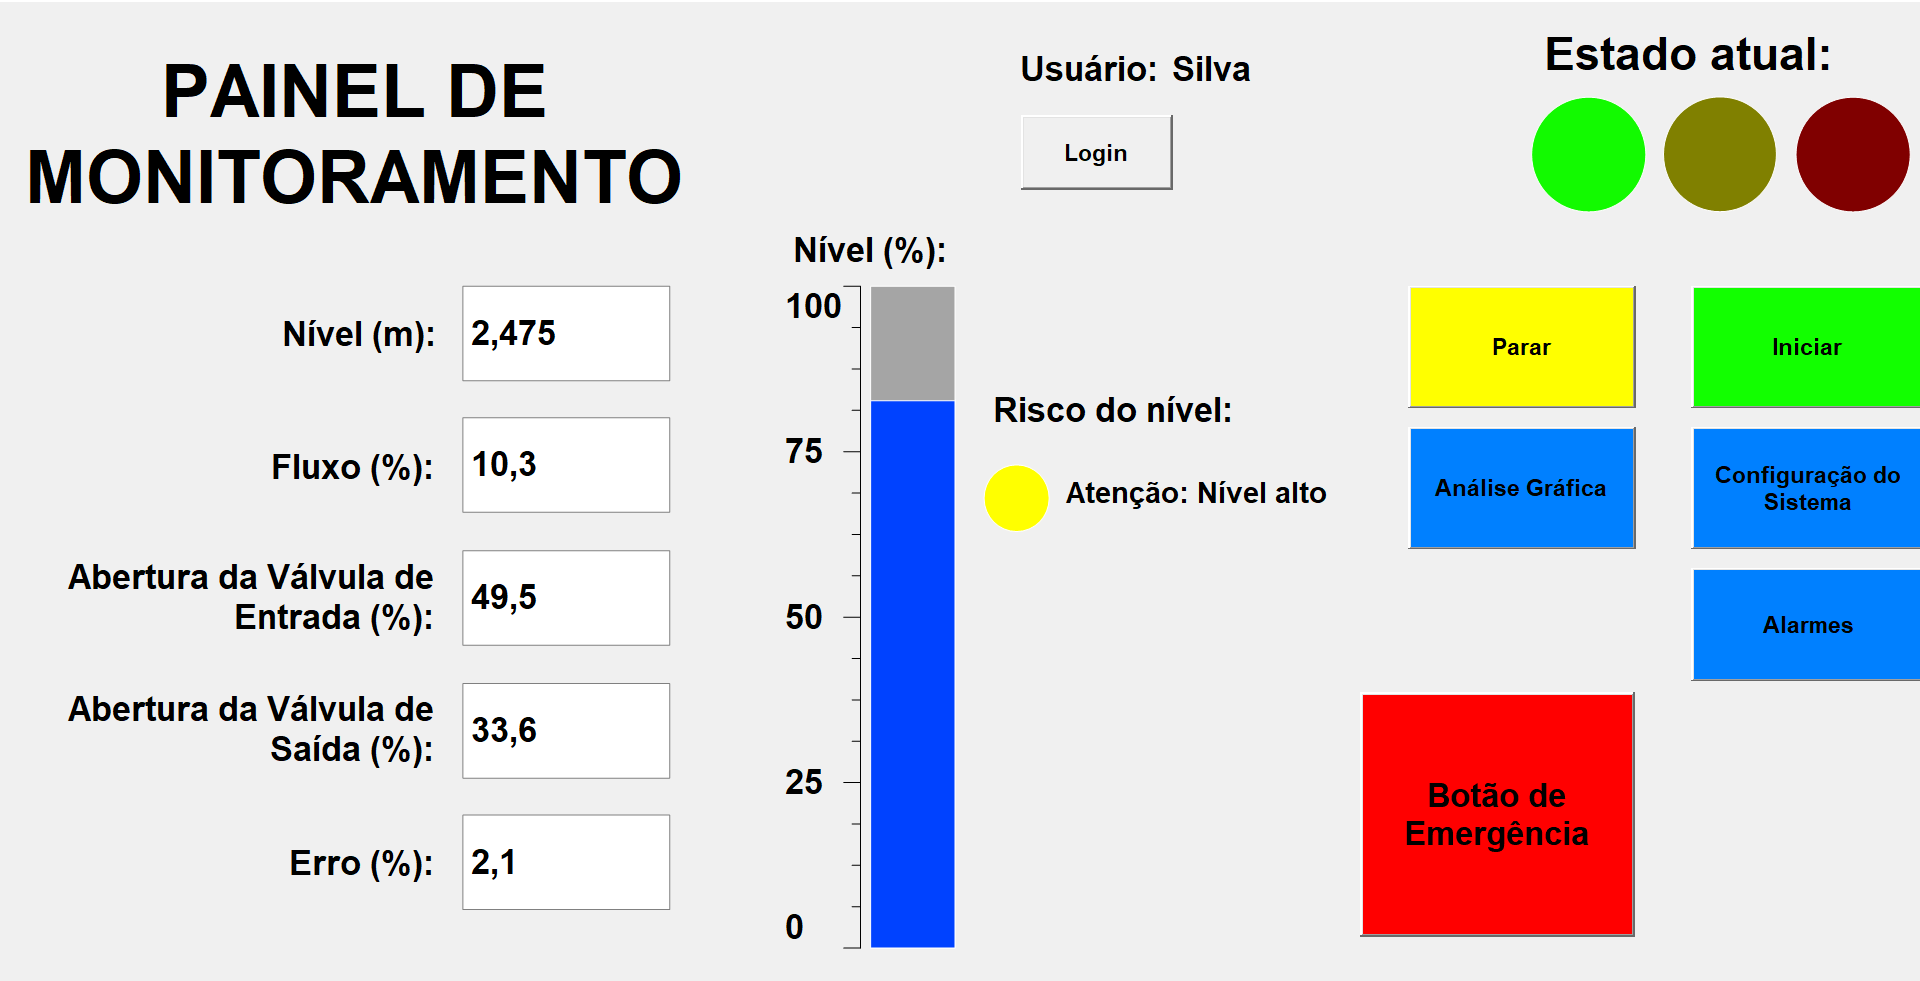
\includegraphics[width=0.8\textwidth]{img/ui_geral.png}
    \label{fig:tel1}
\end{figure}

A segunda tela, chamada Configuração do Sistema, é somente acessível por usuários autorizados, mediante a \textit{login} e senha. Nela é possível realizar diversas alterações no funcionamento do sistema, sendo elas: alteração de ganhos, nível desejado, modo e abertura das válvulas (caso o sistema esteja em manual). Adicionalmente, possui um botão de emergência, os botões de acesso ao gráfico do sistema e ao histórico de alterações, os mostradores para visualizar o valor atual daquilo que se deseja alterar e uma miniatura do gráfico gerado pelo sistema.

\begin{figure}[H]
    \centering
    \caption{Tela de Configuração} 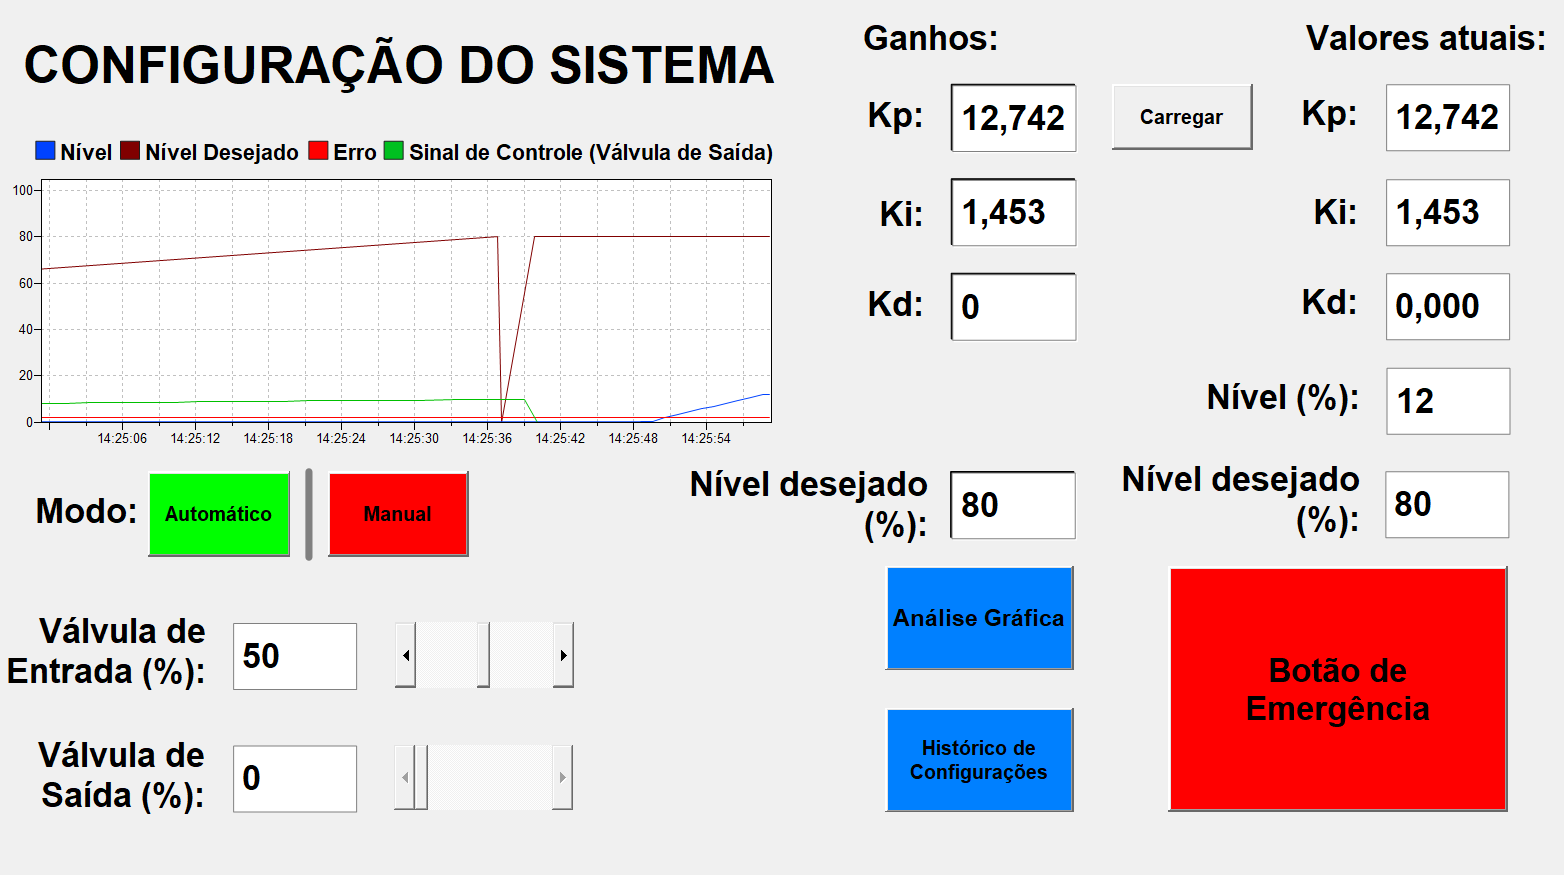
\includegraphics[width=0.8\textwidth]{img/ui_config.png}
    \label{fig:tel2}
\end{figure}

Na tela de Configuração de Alarmes, também restrita a usuários autorizados, podem ser habilitados ou desabilitados os limites do alarme de nível presente no painel de monitoramento, bem como alterar seus valores. Ela possui também uma tabela conectada a um banco de dados, responsável por registrar todos os disparos do alarme, bem como o momento em que foi disparado e o usuário que o configurou.

\begin{figure}[H]
    \centering
    \caption{Tela de Configuração de alarmes} 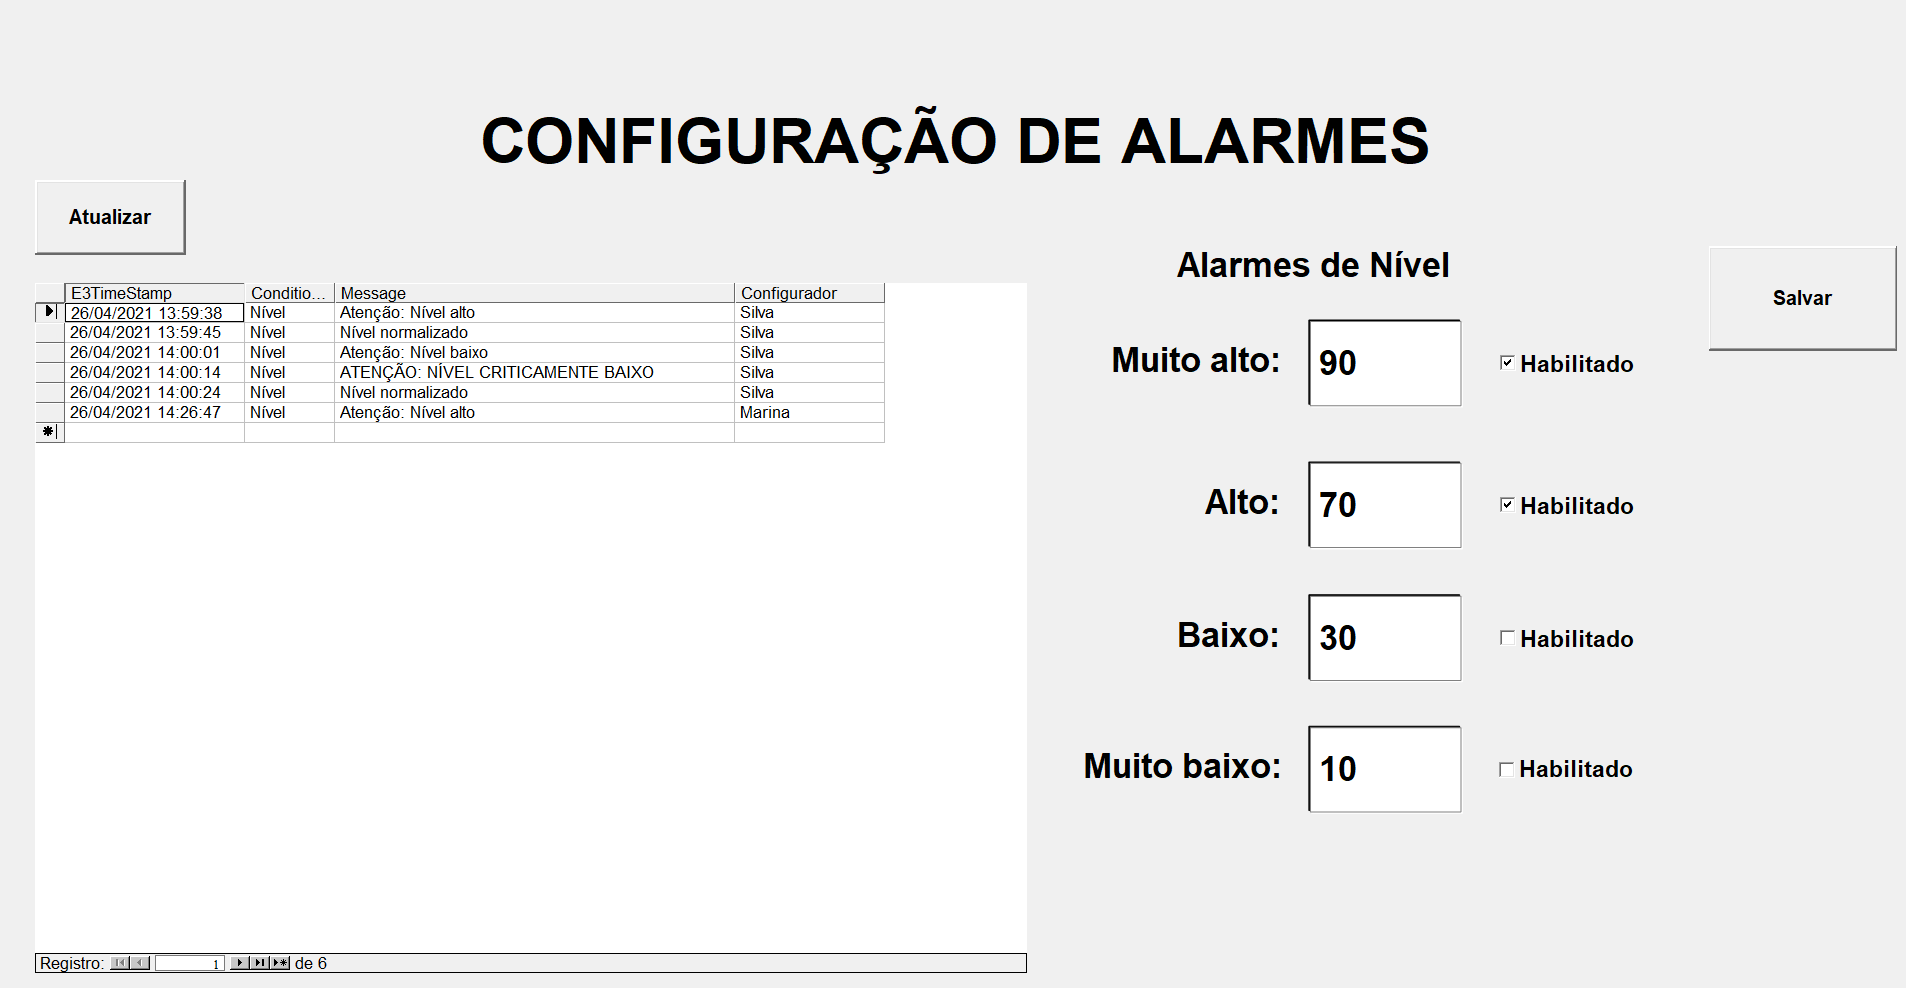
\includegraphics[width=0.8\textwidth]{img/ui_alarm.png}
    \label{fig:ui_alarm}
\end{figure}

A quarta tela é referente ao histórico de alterações nas configurações do sistema e o usuário responsável pelas mesmas, além do histórico de valores essenciais do sistema, como os de nível, fluxo e abertura das válvulas de entrada e saída, sendo atualizado a cada 5 segundos. Ambos os históricos são mostrados em tabelas e estão conectados a seus respectivos bancos de dados.

\begin{figure}[H]
    \centering
    \caption{Tela de Histórico} 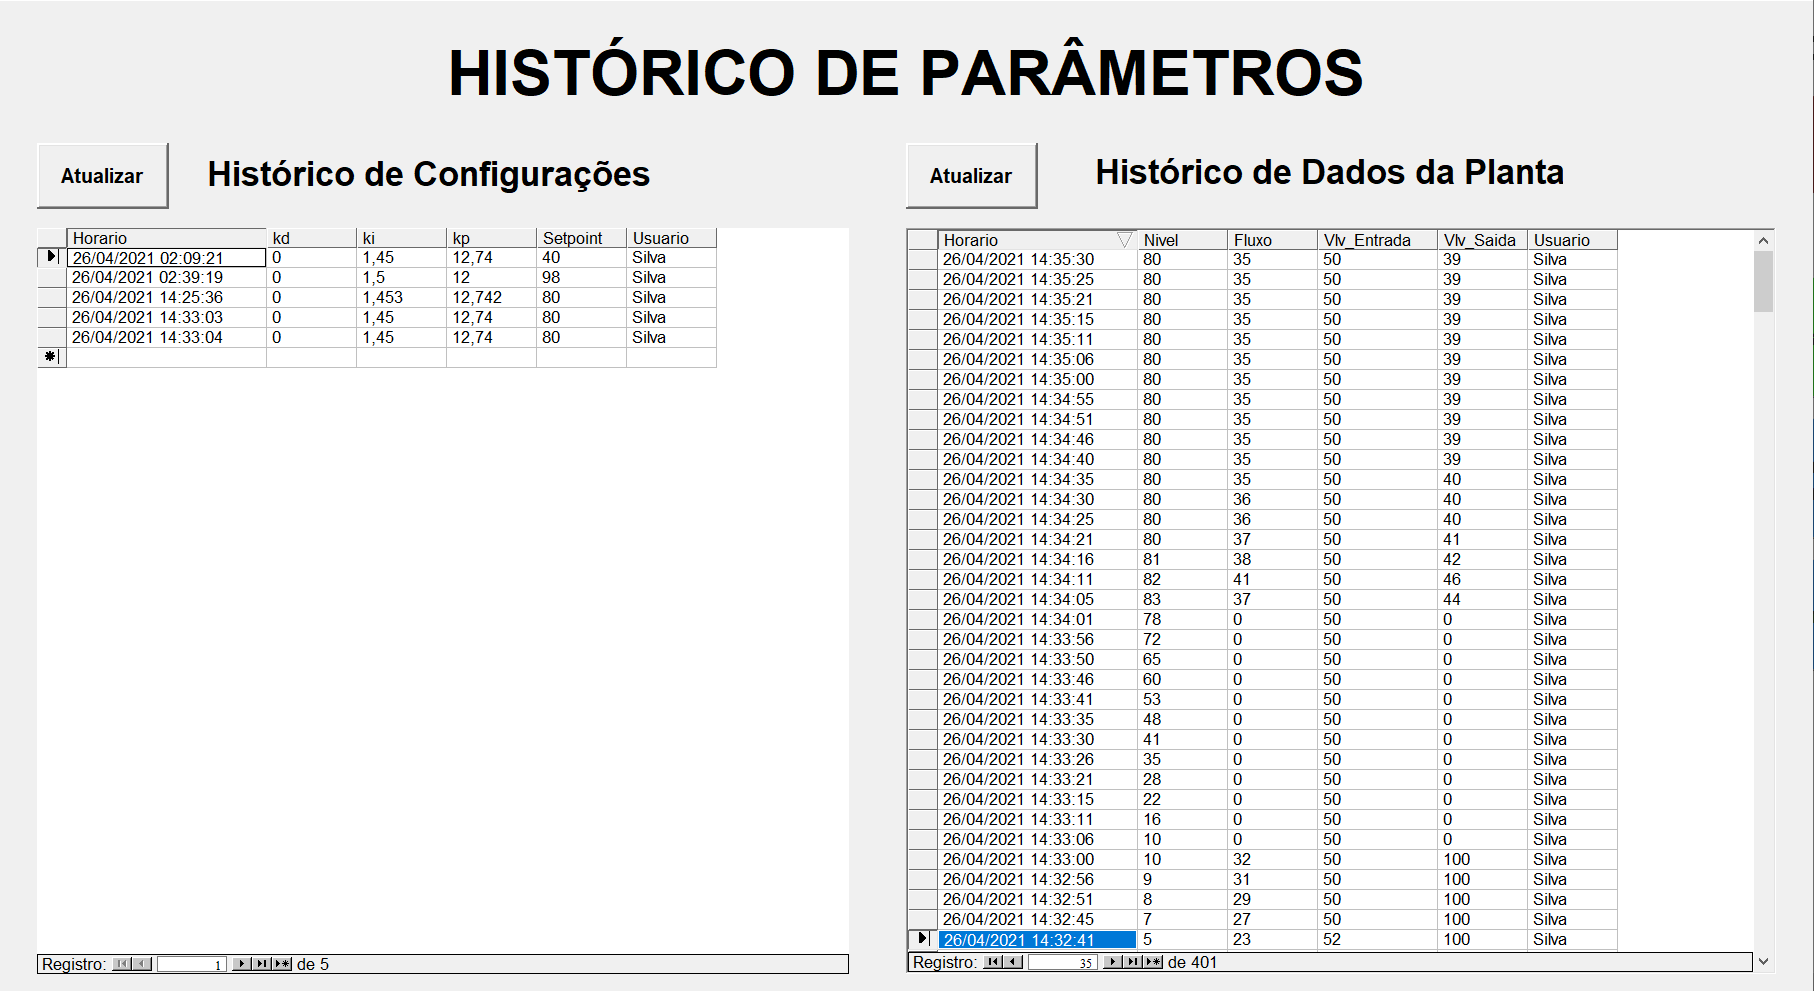
\includegraphics[width=0.8\textwidth]{img/ui_hist.png}
    \label{fig:ui_hist}
\end{figure}

A quinta e última tela, de Análise Gráfica, contém um gráfico gerado em tempo real pelo sistema em função do tempo, demonstrando as curvas relacionadas ao nível atual, ao nível desejado, ao erro e ao sinal de controle (abertura da válvula de saída).

\begin{figure}[H]
    \centering
    \caption{Tela de Análise Gráfica} 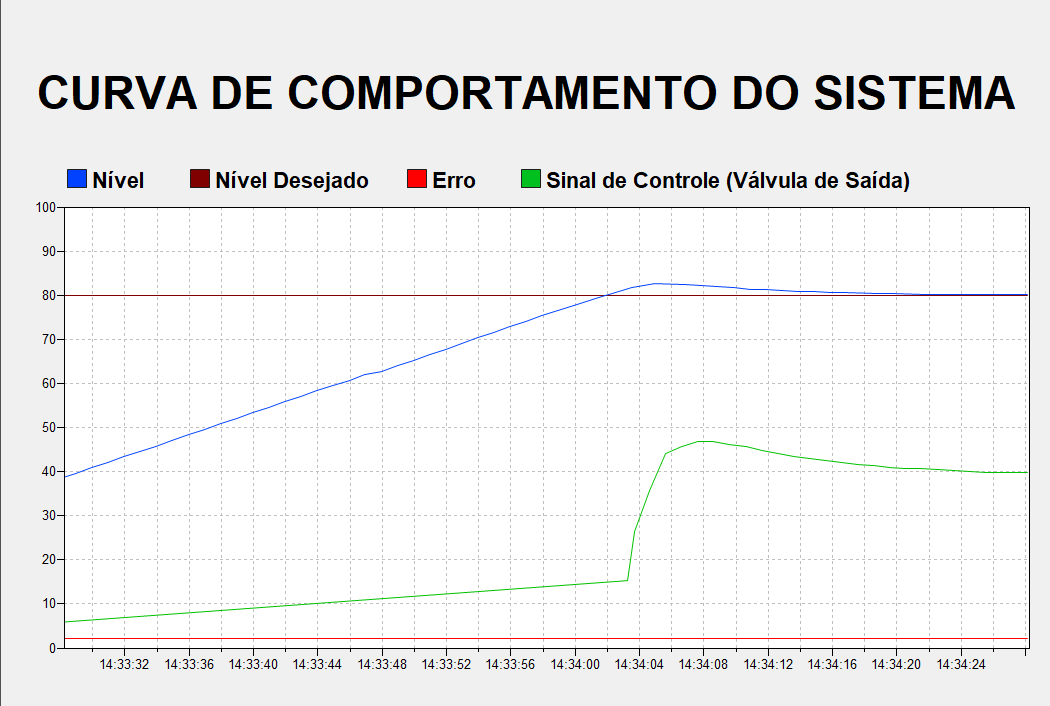
\includegraphics[width=0.8\textwidth]{img/ui_graph.png}
    \label{fig:analise_grafica}
\end{figure}

\subsection{Comunicação}
%Para a comunicação com o \factorio{} foi instalado um driver \textit{modbus} no ambiente do projeto do supervisório, ele utiliza comunicação TCP/IP e possibilita o envio e recebimento de dados através do protocolo \textit{modbus}.
%driver+in/out+registradores+servidor

Para realizar a integração entre a simulação operada pelo \factorio e o supervisório designado no \EE, foi utilizado um servidor programado em \Py{} se comunicando pelo protocolo \Mb, como detalhado anteriormente. Para isso foi instalado e configurado o \textit{driver} \Mb escolhido conforme os critérios já apresentados. Na imagem abaixo está detalhado o esquema de entradas e saídas.

\begin{landscape}
\begin{figure}[H]
    \centering
\caption{Tags de Comunicação entre o \EE e o servidor \Py{}}
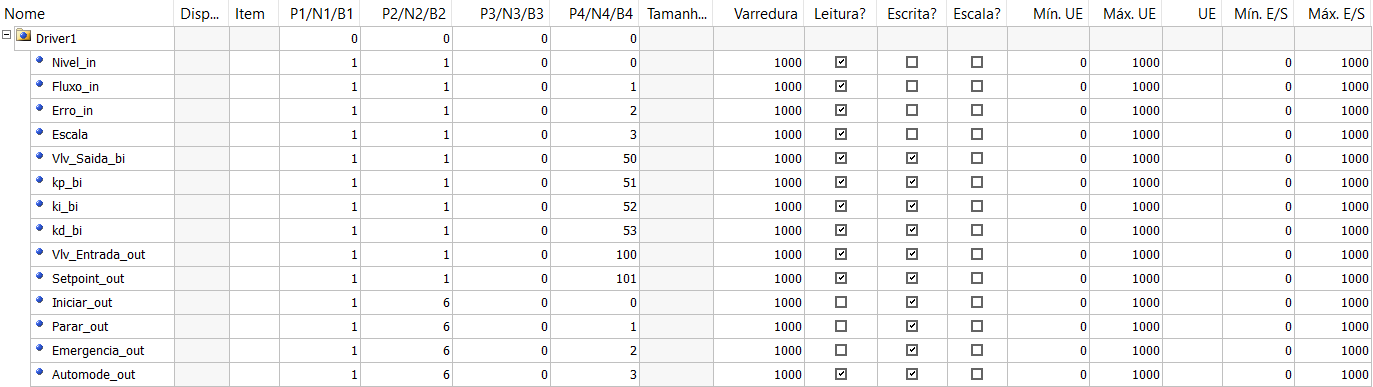
\includegraphics[width=23cm]{img/tags_driver.png}
    \label{fig:tags-comm-2}
\end{figure}

\end{landscape}

\newpage

\section{Conclusão}

Com o projeto concluído, deve-se retomar tudo aquilo que foi feito, desde o entendimento da situação problema, até a montagem de uma solução para operação.
 
O sistema desenvolvido engloba quatro elementos principais: a planta virtual que contém um tanque com sensores de monitoramento e válvulas de entrada e saída; o cliente que simula o controlador de nível da planta; o supervisório para operação do controlador; e o servidor que integra os elementos. Todos as partes se comunicam através do protocolo de rede \Mb, permitindo que cada uma delas opere em uma máquina diferente se for preciso.

Além desses elementos, foi desenvolvido um modelo matemático da planta a partir dos ensaios realizados, permitindo o cálculo dos controladores. Para a operação desse sistema, foram formulados quatro diferentes funções: controlador P, controlador PI, controlador PID e controlador discreto de 1ª ordem. Dos quais o controlador PI se mostrou mais vantajoso.

Dessa forma, esse Projeto Integrador possibilitou uma combinação de modelagem e desenvolvimento matemático, operação da planta e comunicação entre máquinas e com o operador, assim gerando um grande aprendizado prático, mesmo em um projeto feito inteiramente no período de EAD. 

O uso da linguagem em \Py{} aliada aos protocolos de comunicação industrial possibilitou uma solução adaptada ao mercado atual e aprimorável, no entanto resultou em algumas inconsistências e adversidades no processo de troca de informações com a interface do usuário. Assim, em projetos futuros poderia-se utilizar uma interface web para operação e um servidor em nuvem, tornando o sistema ainda mais acessível. 
%\subsection{Comunicação com o controlador}
%\subsubsection{Supervisório}
% \begin{figure}[H]
%     \centering
%     \begin{tikzpicture}
%     \begin{axis}[xlabel=t,
%                  ylabel=$Y$ ]
%     \addplot table [y=level, x=t, ]{valve-log.dat};
%     %\addlegendentry{Esboço de G x T}
%     \end{axis}
%     \end{tikzpicture}
%     \caption{Esboço de Y x t}
%     \label{fig:esboco}
% \end{figure}

\newpage
\section*{Anexos}
Os arquivos anexos estão em uma pasta junto ao arquivo do relatório pdf. Organizados conforme a estrutura abaixo:
\begin{enumerate}[label={Anexo \Roman*:}]
    \item Código para comparação dos modelos - script \texttt{analysis/data-analisys.m}.
    \item Dados da resposta step - arquivo \texttt{analysis/step\_test.csv}.
    \item Programa em \textit{python} para testes da planta e controle simples (testes sem interface) - arquivo \texttt{model/PID.py}.
    \item Planilha contendo dados dos ensaios dos controladores - arquivo \texttt{analysis/Dados dos ensaios dos controladores.ods}.
    \item Simulação da planta - Arquivo de projeto \factorio{}: \texttt{factoryio/Control.io}
    \item Código do supervisório no \EE{} e arquivos associados - pasta \texttt{Supervisorio/}.
    \item Código de controle da planta integração com a interface em \Py{} - pasta \texttt{final/}.
    \item Testes de servidores para comunicação com a interface - pasta \texttt{tests/}.
    %\item Apresentações do projeto (pdf dos slides)
\end{enumerate}

\newpage
\section{Referências Bibliográficas}
\begin{itemize}
\item \href{https://sigaa.ifsc.edu.br/sigaa/portais/discente/discente.jsf#}{Bibliografia externa disponibilizada pelos professores através do Sigaa}
\item \href{https://sigaa.ifsc.edu.br/}{\textit{Slides} de aula com deduções disponibilizadas pelos professores através do Sigaa}
\label{ref:pymodbus}
\item \href{https://github.com/riptideio/pymodbus}{Repositório Oficial Pymodbus} e  \href{https://pymodbus.readthedocs.io/}{Documentação Oficial PyModbus}
\item \href{https://github.com/sourceperl/pyModbusTCP}{Repositório Oficial pyModusTCP}
\item \href{https://github.com/m-lundberg/simple-pid}{Repositório Oficial SimplePID} e \href{https://simple-pid.readthedocs.io/en/latest/}{Documentação Oficial simplePID}

\end{itemize}

% ---
% Finaliza a parte no bookmark do PDF, para que se inicie o bookmark na raiz
% ---
\bookmarksetup{startatroot}% 
% ---

% ----------------------------------------------------------
% ELEMENTOS PÓS-TEXTUAIS
% ----------------------------------------------------------
\postextual

% ----------------------------------------------------------
% Referências bibliográficas
% ----------------------------------------------------------
%\bibliography{abntex2-modelo-references}

% ----------------------------------------------------------
% Glossário
% ----------------------------------------------------------
%
% Há diversas soluções prontas para glossário em LaTeX. 
% Consulte o manual do abnTeX2 para obter sugestões.
%
%\glossary

% ----------------------------------------------------------
% Apêndices
% ----------------------------------------------------------

% ---
% Inicia os apêndices
% ---
%\begin{apendicesenv}

% ----------------------------------------------------------
%\chapter{Nullam elementum urna vel imperdiet sodales elit ipsum pharetra ligula
%ac pretium ante justo a nulla curabitur tristique arcu eu metus}
% ----------------------------------------------------------
%\lipsum[55-56]

%\end{apendicesenv}
% ---

% ----------------------------------------------------------
% Anexos
% ----------------------------------------------------------
\cftinserthook{toc}{AAA}
% ---
% Inicia os anexos
% ---
%\anexos
%\begin{anexosenv}
%
%\newpage
%\chapter{Casa da qualidade}



%\begin{sidewaysfigure}[ht]
%\includegraphics[scale=.8]{casa-da-qualidade}
%\caption{Casa da Qualidade}
%\end{sidewaysfigure}

%\end{anexosenv}

% ----------------------------------------------------------
% Agradecimentos
% ----------------------------------------------------------
%\newpage
%\section*{Agradecimentos}

\end{document}

